%%%%%%%%%%%%%%%%%%%%%%%%%%%%%%%%%%%%%%%%%%%%%%
%
%		My Thesis
%
%		EDOC Template
%		2011
%
%%%%%%%%%%%%%%%%%%%%%%%%%%%%%%%%%%%%%%%%%%%%%%
\documentclass[a4paper,11pt,fleqn]{book}

%%%%%%%%%%%%%%%%%%%%%%%%%%%%%%%%%%%%%%%%%%%%%%
%
%		Thesis Settings
%
%		EDOC Template
%		2011
%
%%%%%%%%%%%%%%%%%%%%%%%%%%%%%%%%%%%%%%%%%%%%%%


\usepackage[T1]{fontenc}
\usepackage[utf8]{inputenc}
\usepackage[french,german,english]{babel}


%%%%%%%%%%%%%%%%%%%%%%%%%%%%%%%%%%%%%%%%%%%%%%%
%% EDOC THESIS TEMPLATE: Variant 1.0 -> Latin modern, large text width&height
%%%%%%%%%%%%%%%%%%%%%%%%%%%%%%%%%%%%%%%%%%%%%%%
%\usepackage{lmodern}
%\usepackage[a4paper,top=22mm,bottom=28mm,inner=35mm,outer=25mm]{geometry}
%%%%%%%%%%%%%%%%%%%%%%%%%%%%%%%%%%%%%%%%%%%%%%%

%%%%%%%%%%%%%%%%%%%%%%%%%%%%%%%%%%%%%%%%%%%%%%
% EDOC THESIS TEMPLATE: Variant 2.0 -> Utopia, Gabarrit A (lighter pages)
%%%%%%%%%%%%%%%%%%%%%%%%%%%%%%%%%%%%%%%%%%%%%%
\usepackage{fourier} % Utopia font-typesetting including mathematical formula compatible with newer TeX-Distributions (>2010)
%\usepackage{utopia} % on older systems -> use this package instead of fourier in combination with mathdesign for better looking results
%\usepackage[adobe-utopia]{mathdesign}
\setlength{\textwidth}{146.8mm} % = 210mm - 37mm - 26.2mm
\setlength{\oddsidemargin}{11.6mm} % 37mm - 1in (from hoffset)
\setlength{\evensidemargin}{0.8mm} % = 26.2mm - 1in (from hoffset)
\setlength{\topmargin}{-2.2mm} % = 0mm -1in + 23.2mm 
\setlength{\textheight}{221.9mm} % = 297mm -29.5mm -31.6mm - 14mm (12 to accomodate footline with pagenumber)
\setlength{\headheight}{14pt}
%%%%%%%%%%%%%%%%%%%%%%%%%%%%%%%%%%%%%%%%%%%%%%



\setlength{\parindent}{0pt}

\usepackage{setspace} % increase interline spacing slightly
\setstretch{1.1}

\makeatletter
\setlength{\@fptop}{0pt}  % for aligning all floating figures/tables etc... to the top margin
\makeatother


\usepackage{graphicx,xcolor}
\graphicspath{{images/}}

\usepackage{subfig}
\usepackage{booktabs}
\usepackage{lipsum}
\usepackage{microtype}
\usepackage{url}
\usepackage[final]{pdfpages}

\usepackage{fancyhdr}
\renewcommand{\sectionmark}[1]{\markright{\thesection\ #1}}
\pagestyle{fancy}
	\fancyhf{}
	\renewcommand{\headrulewidth}{0.4pt}
	\renewcommand{\footrulewidth}{0pt}
	\fancyhead[OR]{\bfseries \nouppercase{\rightmark}}
	\fancyhead[EL]{\bfseries \nouppercase{\leftmark}}
	\fancyfoot[EL,OR]{\thepage}
\fancypagestyle{plain}{
	\fancyhf{}
	\renewcommand{\headrulewidth}{0pt}
	\renewcommand{\footrulewidth}{0pt}
	\fancyfoot[EL,OR]{\thepage}}
\fancypagestyle{addpagenumbersforpdfimports}{
	\fancyhead{}
	\renewcommand{\headrulewidth}{0pt}
	\fancyfoot{}
	\fancyfoot[RO,LE]{\thepage}
}

\usepackage{listings}
\lstset{language=[LaTeX]Tex,tabsize=4, basicstyle=\scriptsize\ttfamily, showstringspaces=false, numbers=left, numberstyle=\tiny, numbersep=10pt, breaklines=true, breakautoindent=true, breakindent=10pt}

\usepackage{hyperref}
\hypersetup{pdfborder={0 0 0},
	colorlinks=true,
	linkcolor=black,
	citecolor=black,
	urlcolor=black}
\urlstyle{same}

\makeatletter
\def\cleardoublepage{\clearpage\if@twoside \ifodd\c@page\else
    \hbox{}
    \thispagestyle{empty}
    \newpage
    \if@twocolumn\hbox{}\newpage\fi\fi\fi}
\makeatother \clearpage{\pagestyle{plain}\cleardoublepage}


%%%%% CHAPTER HEADER %%%%
\usepackage{color}
\usepackage{tikz}
\usepackage[explicit]{titlesec}
\newcommand*\chapterlabel{}
%\renewcommand{\thechapter}{\Roman{chapter}}
\titleformat{\chapter}[display]  % type (section,chapter,etc...) to vary,  shape (eg display-type)
	{\normalfont\bfseries\Huge} % format of the chapter
	{\gdef\chapterlabel{\thechapter\ }}     % the label 
 	{0pt} % separation between label and chapter-title
 	  {\begin{tikzpicture}[remember picture,overlay]
    \node[yshift=-8cm] at (current page.north west)
      {\begin{tikzpicture}[remember picture, overlay]
        \draw[fill=black] (0,0) rectangle(35.5mm,15mm);
        \node[anchor=north east,yshift=-7.2cm,xshift=34mm,minimum height=30mm,inner sep=0mm] at (current page.north west)
        {\parbox[top][30mm][t]{15mm}{\raggedleft $\phantom{\textrm{l}}$\color{white}\chapterlabel}};  %the black l is just to get better base-line alingement
        \node[anchor=north west,yshift=-7.2cm,xshift=37mm,text width=\textwidth,minimum height=30mm,inner sep=0mm] at (current page.north west)
              {\parbox[top][30mm][t]{\textwidth}{\color{black}#1}};
       \end{tikzpicture}
      };
   \end{tikzpicture}
   \gdef\chapterlabel{}
  } % code before the title body

\titlespacing*{\chapter}{0pt}{50pt}{30pt}
\titlespacing*{\section}{0pt}{13.2pt}{*0}  % 13.2pt is line spacing for a text with 11pt font size
\titlespacing*{\subsection}{0pt}{13.2pt}{*0}
\titlespacing*{\subsubsection}{0pt}{13.2pt}{*0}

\newcounter{myparts}
\newcommand*\partlabel{}
\titleformat{\part}[display]  % type (section,chapter,etc...) to vary,  shape (eg display-type)
	{\normalfont\bfseries\Huge} % format of the part
	{\gdef\partlabel{\thepart\ }}     % the label 
 	{0pt} % separation between label and part-title
 	  {\setlength{\unitlength}{20mm}
	  \addtocounter{myparts}{1}
	  \begin{tikzpicture}[remember picture,overlay]
    \node[anchor=north west,xshift=-65mm,yshift=-6.9cm-\value{myparts}*20mm] at (current page.north east) % for unknown reasons: 3mm missing -> 65 instead of 62
      {\begin{tikzpicture}[remember picture, overlay]
        \draw[fill=black] (0,0) rectangle(62mm,20mm);   % -\value{myparts}\unitlength
        \node[anchor=north west,yshift=-6.1cm-\value{myparts}*20mm,xshift=-60.5mm,minimum height=30mm,inner sep=0mm] at (current page.north east)
        {\parbox[top][30mm][t]{55mm}{\raggedright \color{white}Part \partlabel $\phantom{\textrm{l}}$}};  %the phantom l is just to get better base-line alingement
        \node[anchor=north east,yshift=-6.1cm-\value{myparts}*20mm,xshift=-63.5mm,text width=\textwidth,minimum height=30mm,inner sep=0mm] at (current page.north east)
              {\parbox[top][30mm][t]{\textwidth}{\raggedleft \color{black}#1}};
       \end{tikzpicture}
      };
   \end{tikzpicture}
   \gdef\partlabel{}
  } % code before the title body

\usepackage{amsmath}
% Fix the problem with delimiter size caused by fourier and amsmath packages.
\makeatletter
\def\resetMathstrut@{%
  \setbox\z@\hbox{%
    \mathchardef\@tempa\mathcode`\(\relax
      \def\@tempb##1"##2##3{\the\textfont"##3\char"}%
      \expandafter\@tempb\meaning\@tempa \relax
  }%
  \ht\Mathstrutbox@1.2\ht\z@ \dp\Mathstrutbox@1.2\dp\z@
}
\makeatother


%%%%%%%%%%%%%%%%%%%%%%%%%%%%%%%%%%%%%%%%%%%%%%
%
%		Thesis Settings
%		Custom settings
%
%		2011
%
%%%%%%%%%%%%%%%%%%%%%%%%%%%%%%%%%%%%%%%%%%%%%%

%
%   Use this file for your own custom packages, command-definitions, etc...
%


% the following lines are for creating a simplified TO-DO box. However since boites is not per default installed with all latex-distributions, we have removed this example again
% if you want to use it and do not have "boites" installed, you can get it from here: http://www.ctan.org/tex-archive/macros/latex/contrib/boites
%
%\usepackage{boites,boites_exemples}
%\newcommand{\todolist}[1]{\begin{boiteepaisseavecuntitre}{TO DO in this chapter} #1 \end{boiteepaisseavecuntitre}}  % creates a little box
% %\newcommand{\todolist}[1]{}  % to be used when to do is not to be printed
  % place your custom packages, etc... in this file!
\usepackage[backend=bibtex, sorting=none,hyperref=true,style=nature,maxcitenames=99,maxbibnames=999]{biblatex}
\usepackage[nottoc]{tocbibind}
\usepackage{graphicx}

\usepackage{floatrow}
\usepackage{multirow}
\newfloatcommand{capbtabbox}{table}[][\FBwidth]
\newenvironment{changemargin}[2]{%
\begin{list}{}{%
\setlength{\topsep}{0pt}%
\setlength{\leftmargin}{#1}%
\setlength{\rightmargin}{#2}%
\setlength{\listparindent}{\parindent}%
\setlength{\itemindent}{\parindent}%
\setlength{\parsep}{\parskip}%
}%
\item[]}{\end{list}}

\bibliography{biblio}
\usepackage[bottom]{footmisc}
\usepackage{tikz} 
\usetikzlibrary{shapes,arrows}

\tikzstyle{block} = [rectangle, draw, fill=blue!60, 
    text width=5cm, text centered, rounded corners, minimum height=1em,node distance=1.5cm,]
\tikzstyle{decision} = [diamond, draw, fill=yellow!20, 
    text width=2cm,  text badly centered, node distance=3cm, inner sep=0pt]
\tikzstyle{line} = [draw, -latex',line width=0.5mm,]
\tikzstyle{cloud} = [draw, ellipse,fill=red!20, node distance=3cm,
    minimum height=2em]
\usepackage{tabls}

\usepackage{braket}
\usepackage{float}
%%%%%%%%%%%%%%%%%%%%%%%%%%%%%%%%%%%%%%%%%%%%%%
%%%%% HEAD: Book-Begin
%%%%%%%%%%%%%%%%%%%%%%%%%%%%%%%%%%%%%%%%%%%%%%
\begin{document}
\frontmatter
\begin{titlepage}
\begin{center}
%\large
\sffamily


\null\vspace{2cm}
{\huge ASSESSMENT OF COVALENT ORGANIC FRAMEWORK STACKING\\[12pt] } 
%\textcolor{gray}{\small{THIS IS A TEMPORARY TITLE PAGE \\ It will be replaced for the final print by a version \\ provided by the service academique.}}
    
\vfill

\begin{tabular}{cc}
\parbox{0.3\textwidth}{
\includegraphics[width=4cm]{images/EPFL_Logo.pdf}}
&
\parbox{0.7\textwidth}{%
	presented july $22^{nd}$ 2019\\
	to the Faculty of Basic Sciences\\
	Laboratory of Molecular Simulation\\
	program of Master in Molecular and Biological Chemistry\\
%
%	ÉCOLE POLYTECHNIQUE FÉDÉRALE DE LAUSANNE\\
	École Polytechnique Fédérale de Lausanne\\[6pt]
	for the grade of Chemist\\
	by\\ [4pt]
	\null \hspace{3em} Viterbo Victor\\[9pt]
%
\small
Submitted to the jury:\\[4pt]
%
    Prof Berend Smit, president of jury\\
    Prof An Ghysels, external expert\\
    Eng. Andres Ortega Guerrero, supervisor\\
%
Lausanne, EPFL, 2019}
\end{tabular}
\end{center}
\vspace{2cm}
\end{titlepage}




%\cleardoublepage
\thispagestyle{empty}


\vspace*{3cm}

\begin{raggedleft}
    	Wings are a constraint that makes \\
	it possible to fly.\\
     --- Robert Bringhurst\\
\end{raggedleft}

\vspace{4cm}

\begin{center}
    To my parents\dots
\end{center}



\setcounter{page}{0}
%\chapter*{Acknowledgements}
\markboth{Acknowledgements}{Acknowledgements}
\addcontentsline{toc}{chapter}{Acknowledgements}
% put your text here
\lipsum[1-2]

\bigskip
 
\noindent\textit{Lausanne, 12 Mars 2011}
\hfill D.~K.

%\chapter*{Preface}
\markboth{Preface}{Preface}
\addcontentsline{toc}{chapter}{Preface}
% put your text here
A preface is not mandatory. It would typically be written by some other person (eg your thesis director).

\lipsum[1-2]

\bigskip
 
\noindent\textit{Lausanne, 12 Mars 2011}
\hfill T.~D.

%%\begingroup
%\let\cleardoublepage\clearpage


% English abstract
\cleardoublepage
\chapter*{Abstract}
%\markboth{Abstract}{Abstract}
\addcontentsline{toc}{chapter}{Abstract (English/Français/Deutsch)} % adds an entry to the table of contents
% put your text here
\lipsum[1-2]
\vskip0.5cm
Key words: 
%put your text here


% German abstract
\begin{otherlanguage}{german}
\cleardoublepage
\chapter*{Zusammenfassung}
%\markboth{Zusammenfassung}{Zusammenfassung}
% put your text here
\lipsum[1-2]
\vskip0.5cm
Stichwörter: 
%put your text here
\end{otherlanguage}




% French abstract
\begin{otherlanguage}{french}
\cleardoublepage
\chapter*{Résumé}
%\markboth{Résumé}{Résumé}
% put your text here
\lipsum[1-2]
\vskip0.5cm
Mots clefs: 
%put your text here
\end{otherlanguage}


%\endgroup			
%\vfill


\tableofcontents
\cleardoublepage
\phantomsection
\addcontentsline{toc}{chapter}{List of figures} % adds an entry to the table of contents
\listoffigures
\cleardoublepage
\phantomsection
\addcontentsline{toc}{chapter}{List of tables} % adds an entry to the table of contents
\listoftables
% your list of symbols here, if needed.


% space before each new paragraph according to the template guidelines.
%(needs to be after titlepage and frontmatter to keep the table of contents lists short)
\setlength{\parskip}{1em}


%%%%%%%%%%%%%%%%%%%%%%%%%%%%%%%%%%%%%%%%%%%%%%
%%%%% MAIN: The chapters of the thesis
%%%%%%%%%%%%%%%%%%%%%%%%%%%%%%%%%%%%%%%%%%%%%%
\mainmatter
\chapter*{Introduction}
\addcontentsline{toc}{chapter}{Introduction}

Covalent Organic Frameworks (COFs) are a novel class of self-assembled small organic molecules, first synthesized by C\^{o}t\'e et al. in 2005\cite{cote_porous_2005}. The monomers involved in their formations are usually quite rigid due to aromaticity and condense through reversible reactions by forming covalent bonds, which leads to the formation of crystalline nanoporous networks\cite{wu_applications_2017}\cite{Kim2019} and hence homogeneous materials. This leads to materials having low density, high porosity\cite{cote_porous_2005}, and optical properties and are therefore excellent candidates for gas separation and storage\cite{wu_applications_2017}\cite{fan_covalent_2018}, electrical devices\cite{pachfule_porous-organic-framework-templated_2013}\cite{liu_hollow_2013}\cite{kim_covalent_2018}, heterogeneous catalysis\cite{bhadra_triazine_2019}, or light-harvesting\cite{dogru_photoconductive_2013}. The wide variety of applications of these materials led to an explosion of chemical and structural diversity. The Computational-Ready Experimental COF database (CoRE COF), from which the COFs used here are from, was containing 187 COF in 2017\cite{tong_exploring_2017} and 280 in 2018 \cite{tong_computation-ready_2018}.


%Indeed , first COFs were two-dimensional polymers formed by a dehydration condensation reaction of boronic acid ($RB(OH)_2$) into boroxin rings ($R_3(BO)_3$), but now, all type of linker, condensation reactions and structures have appeared like vertical linkers to induce three-dimensional structures; although the latest has not yet found as many applications as 2D ones.

% all the while being easy to functionalize both structurally and chemically,

%Their high crystallinity, compare to most polymers, yield a homogeneous material and hence reliable properties.
%Although 2D COFs are, as of now, the most promising, one main issue still remains: defining their exact crystaline structure. Unlike 3D ones, they can addopt a 
The large variety of COFs available induce the need to find way to estimate its properties in order to compare and optimise their performance for any of the applications mentioned above. To do so, the first step is to establish the exact crystalline structure of the material. Indeed, their properties are strongly dependant on their stacking structure; notably their porosity or electronic properties \cite{xu_dependence_2016} necessary for photo-electronic processes or energy storage. Although this would be straightforward for 3D-COFs because of the low degrees of freedom, such is not the case with 2D-COFs that can adopt a variety of stacking modes. But it is difficult to experimentally assess this property, among other because the amount of material to test induces costs in terms of time, labour and resources, although techniques like Nitrogen isotherms or High-Resolution Transmission Electron Microscopy have been successful in some cases. This limitation would strongly impair the development of COFs. Computational chemistry can hence play a crucial role by proposing a cheap and fast way to estimate the structure of a COF. How to use computational chemistry to properly and efficiently tackle this problem will be the matter of interest here.

%The first solution is to use experimental chemistry but the current protocols and experimental techniques are extremely time-consuming. Considering the number of material that would need to be assessed for any of the applications mentioned above, the total cost in terms of time, labor and resources would limit drastically the potential of COFs. 



%The second solution is to use computational techniques to assess quickly and cheaply a great number of materials.

%Since experimental chemistry would be unable to assess such amounts of structures, in part due to technical limitations like the high sensitivity to defects of x-ray diffraction, and the low crystallinity of these materials. In some cases, High-Resolution Transmission Electron Microscopy was able to give some property like the single layer vector but is unable to asses its stacking. Hence, the advantage of using computational chemistry becomes obvious: it makes it possible to assess the structural property like stacking, in a systematic fashion among a very large number of materials without the need for synthesis. These results can then be used to computationally estimate other properties like density, pore-volume, and even band-gap.

A naive approach to establish the stacking mode would be to start from a given structure and apply a geometry and cell optimization using Density Functional Therory (DFT). This method would not only be expensive in terms of computational costs but bear some severe limitations. Indeed, some COFs' Potential Energy Surface (PES) presents one or more local minimums, that could prevent the simulation from reaching the absolute minima.
The protocol chosen in this work is to establish the full PES for the x,y and z offset from one layer to the next. 
To achieve reasonable accuracy a great number of grid-points needs to be computed which can be very costly if performed with advanced techniques especially when the number of grid-points is consider alongside the amount of materials to test. On the other hand, if the technique used is too inacurate it might miss effects that are determining in the stacking mode. To assess the best compromise between computational cost and precision, several techniques were employed on a diverse set of COFs and their accuracy were compared. These techniques range from classical methods(Lennard-Jones and Coulombic interactions) to Tight-Binding approximation(xTB and DFTB+). Finally, a DFT optimisation was performed to serve as reference to evaluate the performance of the different methods.


%the first step of the calculation is to compute it as accurately as possible to then converge to an exact structure and obtain more complex properties of the material. The problem is now that a fine layer-to-layer x,y,z offset grid is necessary to achieve reasonable accuracy, and accurate calculations are very expensive machine-time-wise, especially when the number of grid-points is put together with the number of materials to test. To alleviate this cost, the solution chosen here is to make a first estimation of the structure using a method as cheap as possible and still gives a useful starting point for more in-depth optimization. In this setting, the work detailed below aims at finding the best compromise between calculations too expensive to be interesting as a pre-screener and the ones not accurate enough to give a useful initial guess for the rest of the treatment. With this idea in mind, different computational technics were tested on a diverse set of COFs to evaluate the complexity of calculations needed to achieve reasonable precision. These technics, from simplest to most elaborate are : the Lennard-Jones potential, Lennard-Jones and Coulombic interactions, DFTB+ \cite{aradi_dftb+_2007} and GFN2-xTB \cite{grimme_robust_2017}\cite{bannwarth_gfn2-xtb_2019}. Finally, the reference optimal structure was obtained obtained using DFT.\cite{hohenberg_inhomogeneous_1964}\cite{kohn_self-consistent_1965}

%Furthermore, by scanning all possible x,y,z offsets from one layer to the next it is possible to asses the crystallinity of the material: a steep, smooth potential would yield high crystallinity while irregularities and flatness in the Potential Energy Surface would yield lower crystallinity. This can be of the utmost importance when aiming at applications like light harvesting where irregularity in the crystalline structure can strongly impair the material's efficiency.

%\chapter{Methodology}
\section{General Considerations}

For this work an algorithm is designed both for Lennard-Jones calculation and the management of the different programs that were used throughout the protocol; an overview of the workflow is displayed in Figure \ref{fig:flowchart1}.
The protocol employed in this work starts with a COF selection from the CoRE COF database. The CIF file is then imported, and data were extracted by the algorithm. A single layer is extracted from the structure and placed at the bottom of the simulation box. The geometry of the polymer is kept the same throughout the process. If the charges were missing, the single-layer is passed through an external charge equilibration routine (see \ref{sec:charge}). Then the list of x and y displacement vectors to be tested, in this case, a 25x25 evenly spaced grid over the unit cell, is generated and distributed among threads. Each of the threads then computes the approximate distance between the two sheets at which the Lennard-Jones (LJ) potential cancels for the x,y point.  A two-stage convergence is used for this purpose to increase the speed and cheapen the calculations : first the COF top layer is be displaced by 0.1 unit-cell at every iteration and the LJ potential is computed. When the energy reaches negative values, the COF starts the process over starting from the last distance to yield positive energy using a 0.01 displacement at each iteration. The starting distance $z_0$ for the z PES is the last point to yield positive energy using that second displacement step. From that initial distance $z_0$, 10 points spaced by 0.01 unit-cell were defined, and the $z_0$ point is stored. For each x,y,z grid-point a copy of the single-layer is generated and shifted by the x,y,z offset. All the offsets were defined in cartesian coordinates, hence a z-shift does not affect the x,y offset. The Lennard-Jones interactions are computed by a built-in function of the algorithm. The two structures were then exported under CIF format to be fed in LAMMPS (for LJ and Coulombic calculations), and XYZ format for calculations with DFTB+ and CP2K's implementation of xTB (for tight-binding approximation calculations). The single point energy were obtained with xTB and DFTB+ using bash scripts and run on the FIDIS EPFL cluster. The main program then collects the energies, find the grid-point with the lowest energy associated and generate the structure associated with that grid-point as CIF file to be finally optimized using CP2K's DFT function.



Each COF is studied using a naive structure (theoretical bond-angles and bond-lengths) and using this same structure relaxed using CP2K's geometry and cell optimization in order to assess the need to relax the structure before going to the calculations of the PES.

\begin{figure}\centering\scalebox{0.8}{
\begin{tikzpicture}[node distance = 1.5cm, auto]\centering
    % Place nodes
    \node [cloud] (start) {start};
    \node [block,below of=start] (db) {COF database};
    \node [block,below of=db] (import) {Import new COF and isolate single layer};
    \node [decision, below of=import](has_chg) {Charge assigned ?};
    \node [block,right of=has_chg] (charges) at (3.5,-6) {Charge equilibration}  ;
    \node [block, below of=has_chg] (xy) at (0,-7) {Pick an x,y offset};
    \node [block, below of=xy] (ELJ0) {Find a $z_0$ offset where $E_{LJ}\simeq0$};
    \node [block, below of=ELJ0] (struct_gen) {Generate a structure using the given x,y,z offset ($z_0<z$)};
    \node [block, below of=struct_gen] (LJ) {Compute Lennard-Jones Potential}; % resulting from interactions between the atoms of the two sheets
    \node [block, below of=LJ] (export) {Export generated structure};
    \node [decision, below of=export] (zover) at (0,-14) {z PES computed ?};
    \node [decision, below of=zover] (allover) at(0,-17.5) {All PES computed ?};
    \node [block,below of=allover] (funcall) at (0,-22) {Process structure though LAMMPS, xTB, DFTB+};
    \node [block, below of=funcall] (collect) {Collect energies and find minimum};
    \node [block, below of=collect] (DFT) {Final optimisation with DFT};
    \node [cloud, below of=DFT] (end) at (0,-25) {end};
  

  \path [line] (start) -- (db);  
  \path [line] (db) -- (import);
  \path [line] (import) -- (has_chg);
  \path [line] (has_chg) -- node {no} (charges);
  \path [line] (has_chg) -- node {yes} (xy);
  \path [line] (charges) -- ++(0,-2.5) -- ++ (-2.4,0);
  \path [line] (xy) -- (ELJ0);
  \path [line] (ELJ0) -- (struct_gen); 
  \path [line] (struct_gen) -- (LJ);
  \path [line] (LJ) -- (export);
  \path [line] (export) -- (zover);
  \path [line] (zover.west) -- ++(-2.2,0.0) -- ++ (0,5.5) -- ++(1,0);
  \path [line] (zover) -- node {yes} (allover);
  \path [line] (allover) -- node {yes} (funcall);
  \path [line] (allover.west) -- ++(-3,0) -- ++ (0,12) -- ++(1.8,0);
  \path [line] (funcall) -- (collect);
  \path [line] (collect) -- (DFT);
  \path [line] (DFT) -- (end);
  %\path [line] (funcall.west) -- ++(-0,-0.1) -- ++(-1.2,0.0) -- ++ (0,7.6) -- ++(1.2,0)  ;
  %\path [line] (funcall.west)  -- ++(0,+0.1) -- ++(-1,0) -- ++ (0,4.4) -- ++(1,0)  ;
  %\path [line] (DFT.west) -- ++(-2,0) -- ++ (0,13.5) -- ++(2,0)  ;
\end{tikzpicture}}
\caption{\textit{Workflow of the project}}
\label{fig:flowchart1}
\end{figure}


\section{Lennard-Jones}
%The Lennard-Jones potential is a classical approximation of non-binding interactions where interaction potential between two elements i and j is given by :
%$$E_{LJ}=4\epsilon_{ij}\left[\left(\frac{\sigma_{ij}}{r_{ij}}\right)^{12}-\left(\frac{\sigma_{ij}}{r_{ij}}\right)^{6}\right]$$
%where and $\epsilon_{ij}$ and $\sigma_{ij}$ are pair-specific parameters. 
%The positive part sands for the repulsion that results from the Pauli exclusion principle and the negative one for the coulombic attraction. The exponents were chosen for computational simplicity.
To asses the complexity of the phenomenon involved in the stacking process of COFs, the Lennard-Jones potential is used as a first approach to simulate the Van der Waals interactions. The parameters used were the Universal Force Field parameters from Rapp\'e et al. \cite{rappe_uff_1992}. Since these parameters are element-specific, a mixing rule is needed to combine the parameters. In our case, the Lorentz-Berthelot mixing rules were used\cite{lorentz_ueber_1881}%, as it is the simplest and most widely used one. It reads as follow:
%$$ \sigma_{ij}=\sqrt{\sigma_i\sigma_j}   $$ and $$ \epsilon_{ij}=\frac{\epsilon_i + \epsilon_j}{2}$$
%where indices i denote an element-specific parameter for element i, and indices $ij$ a pair-specific parameter. $\sigma_i$ and $\epsilon_i$ are the distance to $E_{LJ}=0$ from the nucleus and the depth of the well respectively.
%The parameters used are the Universal Force Field  ones
%, which is among the simplest classical approximations in computational chemistry
The tail correction used here is the truncated-shifted correction :
$$E_{LJ}^{corr}(r)=E_{LJ}(r)+E_{LJ}(r_{cut})$$
Where $E_{LJ}^{corr}(r)$ is the corrected potential, and $r_cut$ is the cutoff radius; it ensures a smooth potential at cutoff.

\section{Charge Calculations}
\label{sec:charge}
For the experimental structures (naive bond angle and bond length), no charges were provided and where hence computed for a single sheet using the charge equilibration from EGULP subroutine \cite{kadantsev_fast_2013}. This method is also based on the Universal Force Field's parameters. The core principle behind this method is to use a second-order Taylor expansion, truncated to the second-order, of the charge dependant energy ($E(Q)$)\cite{rappe_charge_1991} :
%$$E_A(Q)=E_{A0}+Q_A\left(\frac{\partial E}{\partial Q}\right)_{A0}+\frac{1}{2}Q_{A0}^2\left(\frac{\partial^2 E}{\partial Q^2}\right)_{A0}$$
This parametrization makes this problem computationally cheap by avoiding to go through a long and tedious quantum processing of the system and hence fast charge equilibration.

Calculations were performed on a single sheet to exclude Coulombic interactions between layers.

% Unfortunately, this method was not robust enough and showed some unphysical behaviors, among others yielding strongly asymmetric charge distribution in a symmetric system or yielding positively charged Fluorine in fluorinated benzene. This indicates that the systems under study here need to be dealt with more advanced techniques to obtain the equilibrated charges. Hence 

The charges were also computed using DFT with the parameters detailed in section% \ref{sec:dft}

The charge density was partitioned using either the Hirshfeld method \cite{hirshfeld_bonded-atom_1977} or the Density Derived Electrostatic and Chemical (DDEC) charge method \cite{manz_chemically_2010}.

An in-depth analysis of the charges as computed by DFTB+ is also performed to asses the strength of the interactions between layers in the repartition of charges. This may enable one to estimate the correlation between charge distribution and stacking and hence the necessity to recompute the charges for every configuration or not. 



\section{Coulombic Potential and Ewald Summation}

%The Coulombic potential is given by :
%$$E_c=k_e\frac{q_iq_j}{r_{ij}}$$
%where $k_e$ is the Coulomb's constant, $q_i$ and $q_j$ the charge of the atoms i and j respectively, and $r_{ij}$ the distance between the two atoms. 
%Since the potential converges slowly in periodic systems, it is important to take into account the long-range interactions. A natural way to do so would be to use a very high cutoff but it would increase the computational cost drastically. To tackle this problem, one can take advantage of the periodicity of the system and compute separately the short-range interactions by summing them in real space and sum the long-range interactions in reciprocal space: this is known as the Ewald summation, which is a special case of the Poisson summation. The charge density is split as follow :
%$$\rho_i(r) = \rho_i^S(r)+\rho_i^L(r)$$
%where $\rho_i^S(r)$, the short-range function is as follow
%$$\rho_i^S(r) = q_i\delta(r-r_i)-q_iG_\sigma(r-r_i)$$
%and $\rho_i^L(r)$, the long-range function :
%$$\rho_i^L(r)=q_iG_\sigma(r-r_i)$$
%with 
%$$G_\sigma=\frac{1}{(2\pi\sigma^2)^{3/2}}exp\left[-\frac{|r|^2}{2\sigma^2}\right]$$
%The substitution above is equivalent to adding and subtracting a Gaussian function around each point charge, described by a Dirac delta function. This will shield long-range interactions in the short-range function and is corrected by the long-range function to maintain a correct description of the physical system.
%We then integrate the short-range function in real space and the long-range in reciprocal space.
Since our problem is a periodic system, the convergence of the Coulombic potential is achieved using the Ewald summation\cite{lee_ewald_nodate}. For this project, LAMMPS (Large Scale Atomic/Molecular Massively Parallel Simulator)\cite{plimpton_fast_nodate} is used for its implementation of the Particle-Particle-Particle-Mesh Ewald Summation (PPPM) \cite{hockney_computer_1981} , with a threshold of $10^{-6}$ $kcal/mol$.
Only interactions between two designated sets of atoms, here the two layers, were computed and hence neglecting the intra-layer interactions
% To be able to grasp the principle of the two following technics, it is important to first go through the principle that is the foundation of almost all newly developed technics: the Density Functional Theory. It mostly lies on the Hohnenberg-Kohn theorem that states that : 

%\textit{In a finite, interacting N-electron system with a given particle-particle interaction, there exists a one-to-one correspondence between the external potential v(r) and the ground state-density $n_0[v](r)$. In other words, the external potential is a unique functional of the ground-state density, $v[n_0](r)$, up to an arbitrary constant}\cite{ullrich_time-dependent_2011}. 

%With :
%$$n_0[v](r)=\sum_i|\Psi_i(r)|^2$$

%This equivalence simplify greatly the calculations and enabled computational chemistry to start tackling problems of a complexity that was before out of reach. The difficulty now resides in finding an efficient functional to compute the energy and other system properties.



% It lies on the equivalence between treating $N$ one-electron wavefunction $\Psi_i$ and one $N$ electron density function $n(r)$ with :
%where the summation is done over the $i$ electrons.
%It is based on the fact that a non-degenerate ground state of a $N$ electron system is fully determined for a given external potential, and hence :
%$$V_{ext} \leftrightarrow n(r)$$
%The first Hohnenberg-Kohn theorem goes further and state that a unique functional of the density function $n(r)$ exists and yield the energy of the system.
%The second Hohnenberg-Kohn theorem state that the true density function of the ground state is the one that minimizes the energy.
%Together these theorems are the foundation of DFT calculations.

For the CP2K relaxed structures, the charges were provided as computed by DFT in the two-layer structure provided.

 
\section{Geometry, Frequency, Non-bonding - Tight Binding method (GFN2-xTB)}

GFN2-xTB is a Tight-Binding approximation with atom-specific parametrization. For the purpose of this project, the CP2K delvopment version of this algorithm was used with the D3 dispersion correction and the SPME (Smooth Particle Mesh Ewald) summation, the Hessian matrix is estimated using the Broyden mixing scheme using the last 8 steps and was alternated with the Direct Inversion in the Iterative Subspace \cite{pulay_convergence_1980}\cite{pulay_improved_1982}\cite{shepard_comments_2007}. The threshold for SCC conversion used is $10^{-6}$ and the D3 correction for dispersion%It is mostly designed for vibrational analysis, geometry optimization and non-covalent interactions (the latest being the one of interest here).
%The theory it relies on reads as follow, starting from the total energy :
%$$E=E_{el} + E_{rep} + E_{disp} + E_{XB}$$
%with $E_{rep} $ the repulsion energy, $E_{disp}$ the dispersion energy and $E_{XB}$ the halogen bonding and $E_{el}$ the electronic potential is based on a corrected third-order-truncated Taylor expansion of the Hamiltonian :
%$$E_{el}=\sum_i^{occ}n_i\braket{\Psi_i|H_0|\Psi_i}+\frac{1}{2}\sum_{A,B}\sum_{l(A)}\sum_{l'(B)}p_{l}^Ap_{l'}^B\gamma_{AB,ll'}+\frac{1}{3}\sum_A\Gamma_{A}q_A^3-T_{el}S_{el}$$
%The first order therm is simply the energy associated with each electron in its Molecular Orbital, the second order and third order term are the SCC contribution taking only in account diagonal terms and the additional term $T_{el}S_{el}$ is the electronic thermal-entropic terms.
 
 %$\Psi_i$ is the valence Molecular Orbital with occupation $n_i$, $H_0$ the zero-order Hamiltonian, $q_A$ the Mulliken charges of atom $A$, $\Gamma_A$ the derivative of the Hubbard parameter $\eta_A$,$l$ and $l'$ are the electronic shells of atoms $A$ and $B$ respectively and $p_l^A$ the charge distribution on atom $A$'s shells with angular momentum $l$  and $\gamma_{AB,ll'}$ is a Coulombic space-dependant damping factor.

%xTB is run on CP2K's development version


\section{DFTB+}
The Density Functional-Based Tight Binding (DFTB) implemented on DFTB+ program is a more heavily parameterized method. Like xTB, it relies on an expansion around the density-functional energy but uses atomic parametrisation for the electronic Hamiltonian diagonal terms (element-specific) as well as for the off-diagonal ones (pair specific).
For this process, were used two sets of parameters : the 3ob-3-1 (parametrisation for Organic and Biological System) set \cite{kubillus_parameterization_2015}\cite{lu_parametrization_2015}\cite{gaus_parameterization_2014}\cite{gaus_parametrization_2013} and the Matsci-0-3 \cite{frenzel_semirelativistic_nodate} (parametrisation for Material Sciences) set for COFs containing Boron (COF-1 and COF-5). The two sets of parameters were compared for a COF were both sets could be used.
The static grid-point calculations were performed with a self-consistent Hamiltonian, with a force and self-consistency threshold of $10^{-5} a.u$, the Broyden mixer is used, and the k-points were set to x,y,z=\{1,1,1\}, the D3 method using the Becke-Johnson damping factor and including the Hubbard derivatives is used for dispersion correction and damped in the special case of Hydrogen to mimic Hydrogen-bonding.

The cell and geometry optimization is performed using the same parameters except with a lower threshold for the forces and SCC: $10^{-6}$. 

%It is based on the spin-polarized Hamiltonian below :
%$$\hat{H}_{\mu\nu}^\sigma = \braket{\phi_\mu|\hat{H_0}|\phi_\mu}+\frac{1}{2}S_{\mu\nu}\sum_C\sum_{l''\inC}(\gamma_{Al,Cl''}+\gamma_{Bl',Cl''})\Delta q_{C_{l''}}$$
%$$\pm \frac{1}{2}S_{\mu\nu}\left(\sum_{l''\in A}W_{All''}m_{Al''}+\sum_{l''\in B}W_{Bll''}m_{Bl''}\right)$$
%The first term being the non-SCC Hamiltonian, the second term is the SCC contribution,



\section{Density Functional Theory}
\label{sec:dft}
%Density Functional Theory is a technique relying on the physical equivalence of a set of $N$ one-electron wavefunction $\Psi(r)$ and the sum of its position dependent module $n(r)$, the density function. A functional is then applied to the density function to extract observables as the energy. It was here used as the last stage of our process to obtain the reference COF stacking starting from each technique's guess to asses its accuracy. The parameters used were the same as for the charge equilibrations.

The charge calculations using DFT were performed with PBE (Perdew$-$Burke$-$Ernzerhof), a nonempirical GGA (Generalized Gradient Approximation) functional and Self-Consistency Field (SCF) is enforced using DIIS minimizer (Direct Inversion in Iterative Subspace) \cite{pulay_convergence_1980}\cite{pulay_improved_1982}\cite{shepard_comments_2007} with a threshold of $10^{-6}$. The DFT-D3 correction term for dispersion forces (London Forces) is used and set to include the $9^{nth}$ order term since these play a key role in the non-bonding interactions which will determine the optimum stacking. For all elements, including Hydrogen, a Gaussian Double-Zeta function is used for the basis set \cite{vandevondele_gaussian_2007} to mimic accurately polarisation.

The geometry and cell optimisations were performed with the same method as for the charge optimisation, no symmetry constrains nor external pressure were applied and with the Broyden–Fletcher–Goldfarb–Shanno (BFGS) optimiser, a type of steepest descant optimizer.

\section{COF sample}
In order to assess the different phenomenons that intervene in the stacking process of Covalent Organic Frameworks, a chemically and structurally diverse set of COFs was chosen. they are represented on Figure \ref{fig:struct}. The two first ones are among the first synthesized COFs by Cot\'e et al., the first is made by cyclic condensation of boronic acids. The second one by condensation of boronic acid and di-alcool. The third fourth and fifth by triazine cyclic condensation and the last one by imine condensation. The first fourth are flat COF the fifth one is non-flat because of the methyl groups and the sixth one is slightly V-shaped because of the steric hindrance of the Hydrogens between the benzene and the pyrene; this curvature induces a strain on the pyrene and break aromaticity.

\begin{figure}[H]

%\caption[A floating table]{Structures of the COFs under study}

\centering
\begin{tabular}{cc}
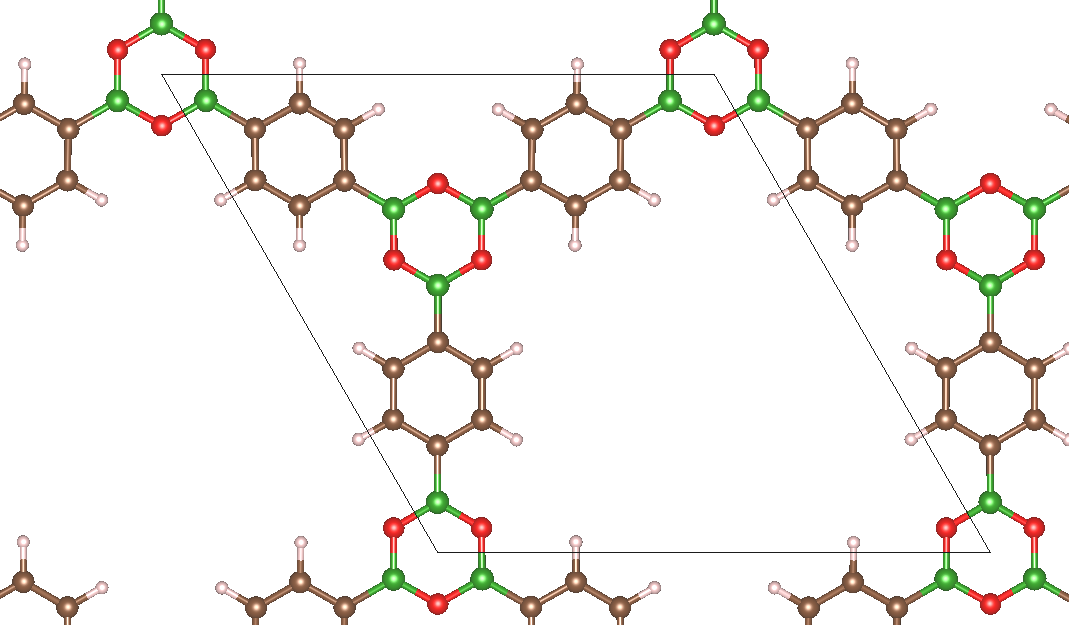
\includegraphics[height=4cm]{images/05000.png} & 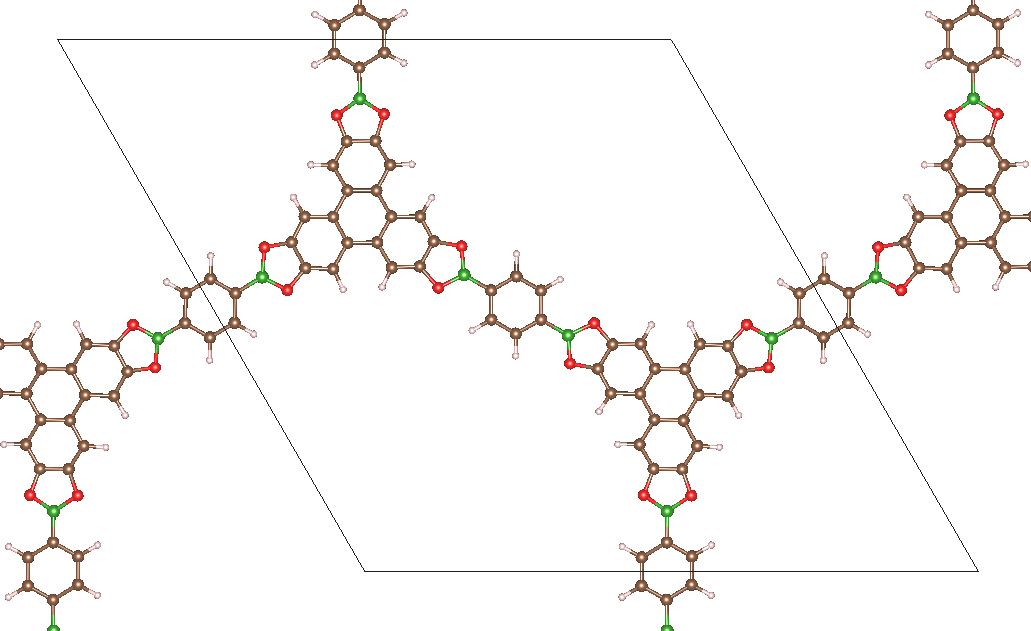
\includegraphics[height=4cm]{images/050001.png} \\ 
\textbf{05000N2}\par\medskip & \textbf{05001N2}\par\medskip\\
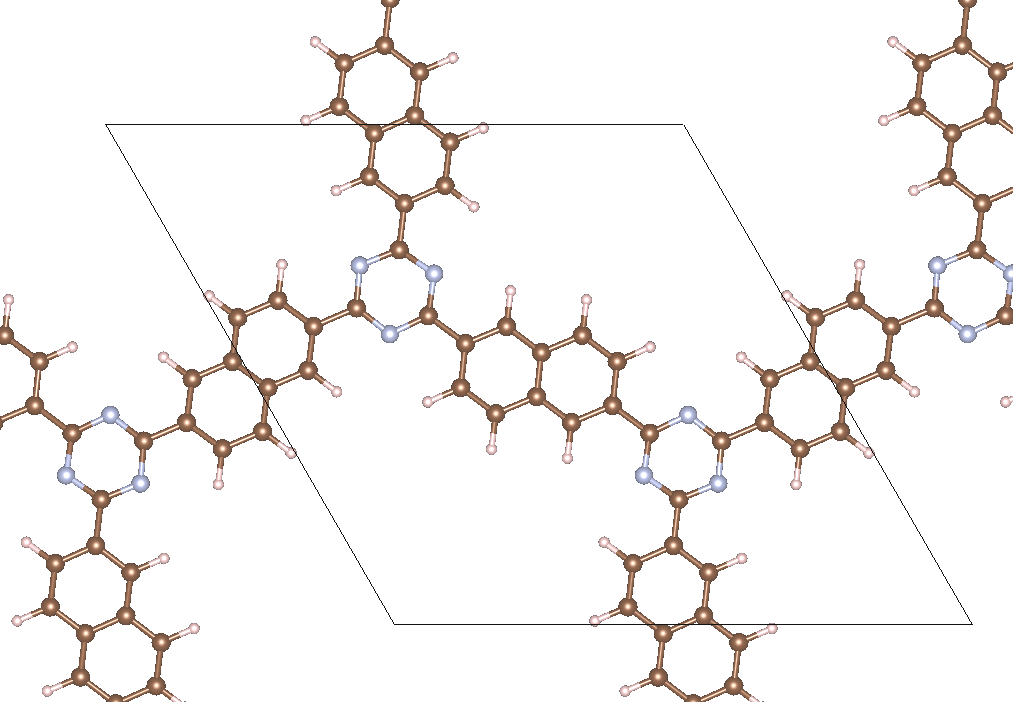
\includegraphics[height=4cm]{images/10000.png} & 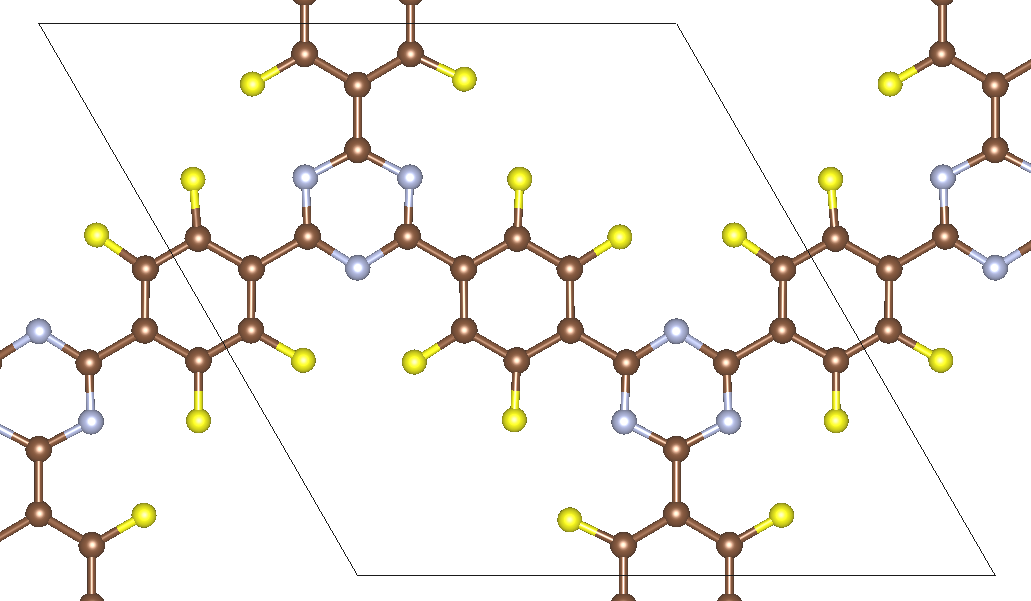
\includegraphics[height=4cm]{images/13000.png} \\
\textbf{10000N2}\par\medskip & \textbf{13000N2}\par\medskip\\
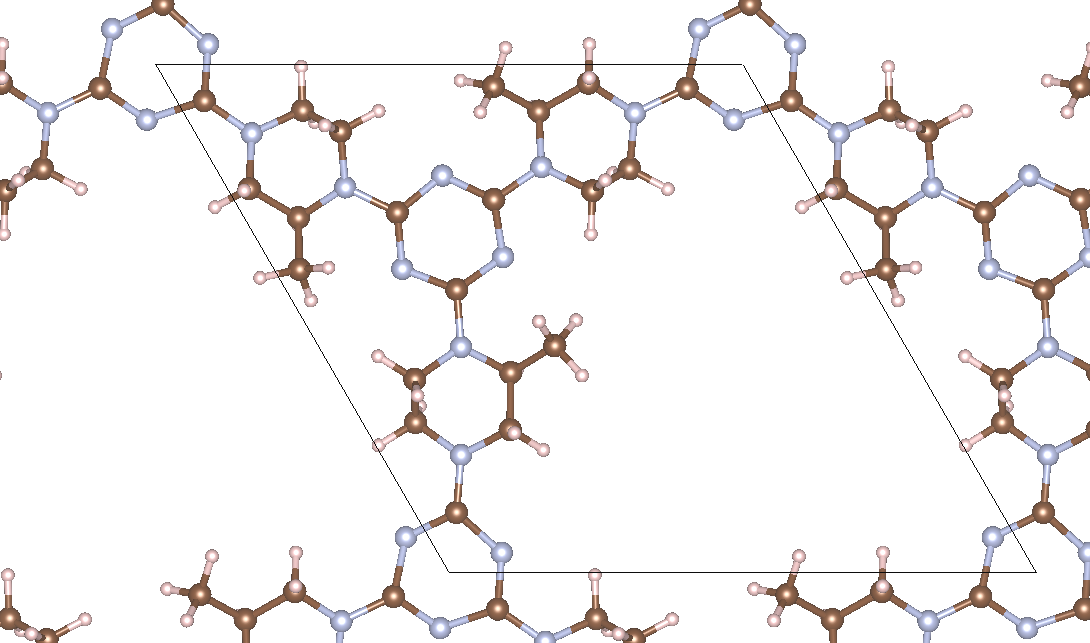
\includegraphics[height=4cm]{images/17120.png} & 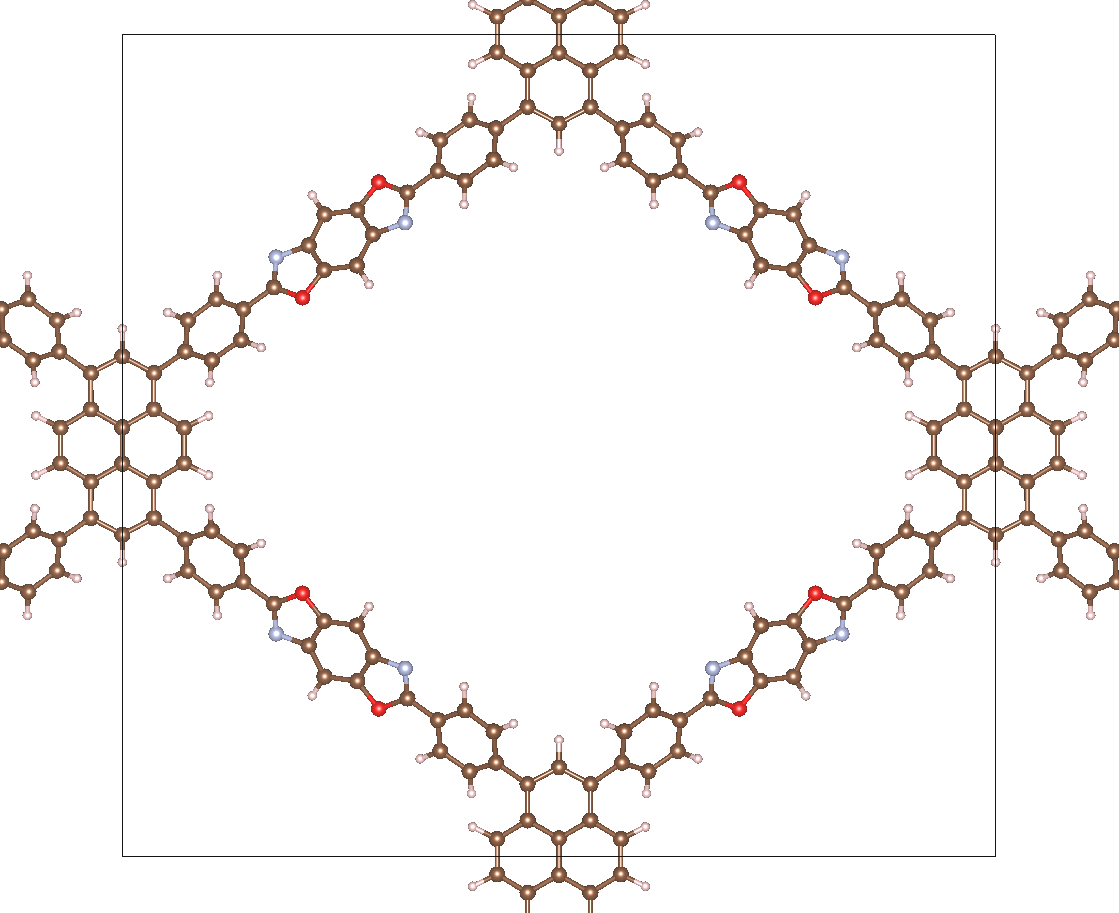
\includegraphics[height=4cm]{images/18112.png} \\ 
\textbf{17120N2}\par\medskip & \textbf{18112}\par\medskip\\
\end{tabular}
\caption{Structure of COFs studied in this work; from left to right and top to bottom; Carbon in brown, Oxygen in red, Hydrogen in white, Boron in green, Nitrogen in blue, Fluorine in yellow}
\label{fig:struct}
\end{figure}


\chapter{Results}

%COFs with high conformational degrees of freedom (like alkyl chain) were purposely excluded from the set since they are not well suited for the type of calculations performed here and should be treated differently using a different approach.


\section{Preliminary tests}
All preliminary test were performed by establishing the potential along the z axis on COF1 without x and y offsets between the sheets.

\subsection{Lennard-Jones}
Since the Lennard-Jones potential was implemented as a built-in function and not using an established program, a benchmarking was performed using the Lennard-Jones implementation of LAMMPS as a reference. The results are displayed on Figure \ref{fig:lj_bench}

\begin{figure}%[H]
\centering
\begin{tabular}{cr}
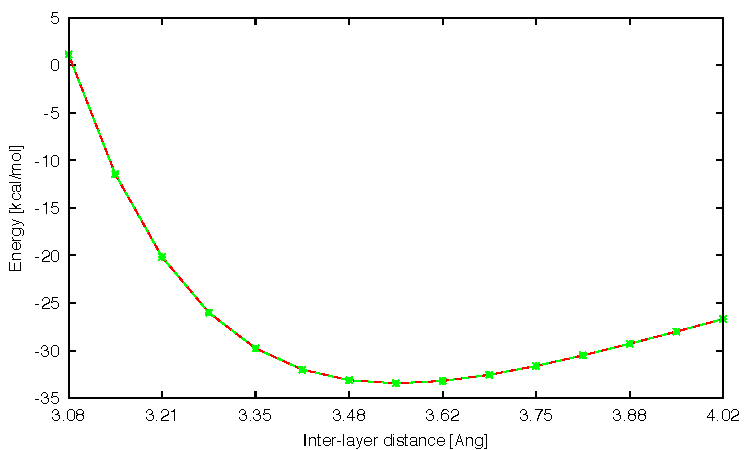
\includegraphics[width=6cm]{images/bench_lj.pdf}&  
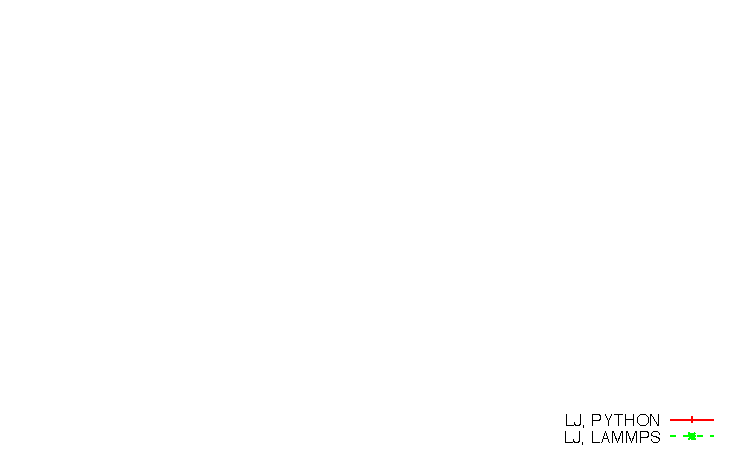
\includegraphics{images/key_bench_lj.pdf}\\
\end{tabular}
\caption{Comparison of the Lennard-Jones potential computed using our program and LAMMPS using a cutoff of 15$\AA$  and no tail correction}
\label{fig:lj_bench}
\end{figure}

The conclusion was that the Lennard-Jones potential was correctly implemented in the algorithm.




\begin{samepage}


Then a convergence test was performed to estimate the necessary cutoff. The potential obtained using different cutoffs are displayed on Figure \ref{fig:LJ_conv}

\begin{figure}[H]
\centering
\begin{tabular}{cr}
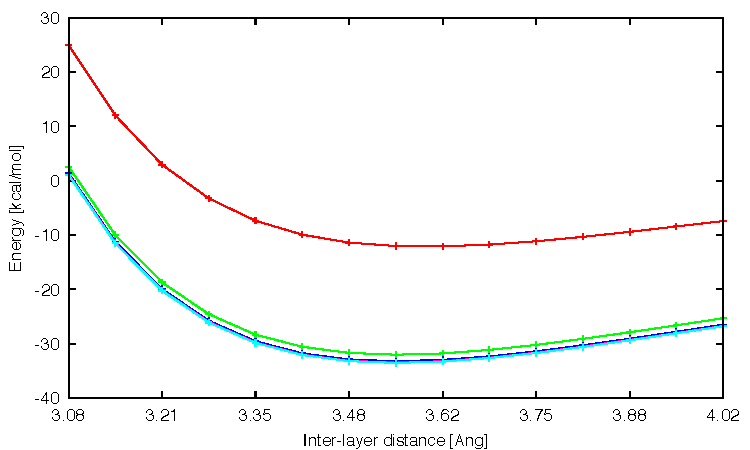
\includegraphics[width=6cm]{images/LJ_conv.pdf}& 
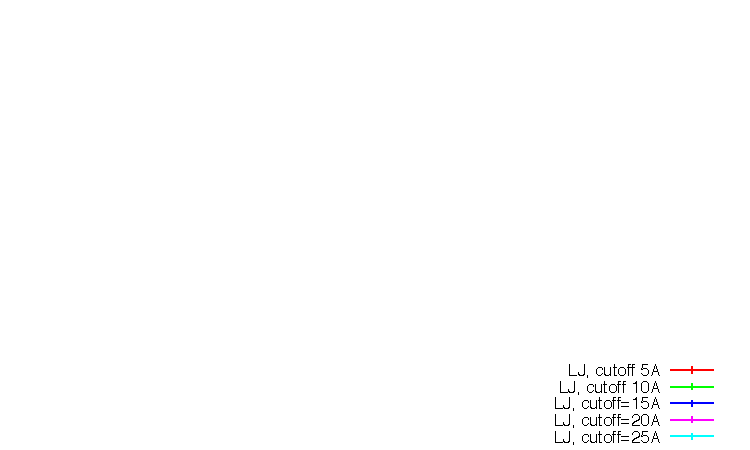
\includegraphics{images/key_lj.pdf} \\
\end{tabular}
\caption{Comparison of the Lennard-Jones potential as a function of the cutoff in $\AA$}
\label{fig:LJ_conv}
\end{figure}

From this, the conclusion was that a cutoff of 15 $\AA$ was sufficient.
\end{samepage}


\begin{samepage}

\subsection{Coulombic interactions}

As a first attempt, the coulombic interaction was also implemented as a built-in function with different tail corrections and damping functions, the Ewald summation implemented on LAMMPS was used as the reference. The results are displayed on Figure \ref{fig:coul_conv}

\begin{figure}[H]
\centering
\begin{tabular}{cr}
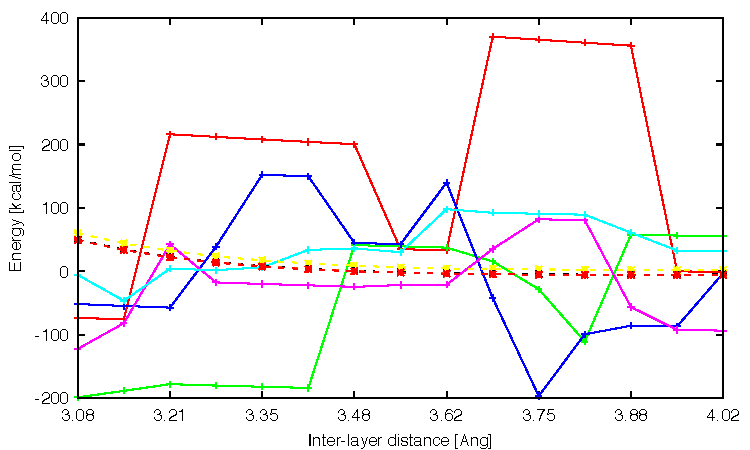
\includegraphics[width=6cm]{images/Coul_conv.pdf}&
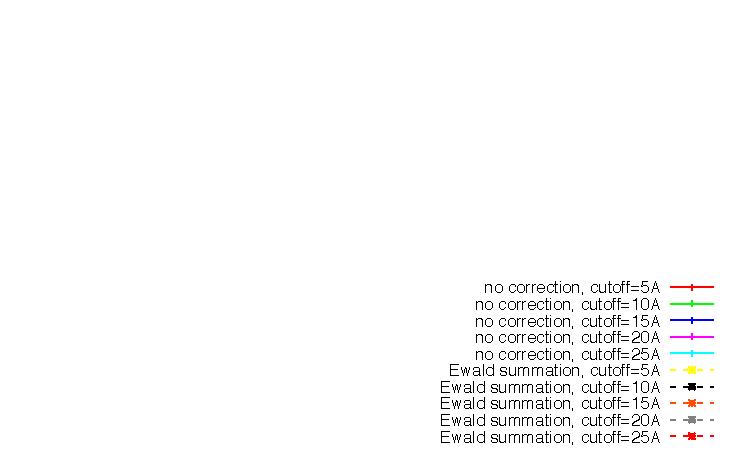
\includegraphics{images/key.pdf} \\
\end{tabular}
\caption{Comparison of the coulombic potentials with and without correction.}
\label{fig:coul_conv}
\end{figure}

\end{samepage}

\section{Stacking assessment and PESs}
\begin{figure}%[H]
\centering
\begin{tabular}{|c||c|c|c|c|c|c|}
\hline
COF & axis & LJ & LJ+Coul. & xTB & DFTB+ & DFT\\
\hline
\hline
\multirow{3}{*}[-0.3cm]{05000N2}&x&-1.88&-16.28&$/^*$&-2.50&-4.06\\
\cline{2-7}
&y&-8.68&8.68&$/^*$&0&-3.02\\
\cline{2-7}
&z&3.22&3.15&$/^*$&2.95&3.63\\
\hline
\hline
\multirow{3}{*}[-0.3cm]{05001N2}&x&3.00&-1.19&$/^*$&-1.19&-2.43\\
\cline{2-7}
&y&8.23&6.17&$/^*$&-2.06&-4.20\\
\cline{2-7}
&z&3.32&3.39&$/^*$&2.98&3.42\\
\hline
\hline
\multirow{3}{*}[-0.3cm]{10000N2}&x&0.73&2.94&-0.73&0&-3.88\\
\cline{2-7}
&y&-1.27&-2.54&-3.82&2.54&2.79\\
\cline{2-7}
&z&3.43&3.42&3.23&3.02&3.43\\
\hline
\hline
\multirow{3}{*}[-0.3cm]{13000N2}&x&-1.75&-13.41&15.74&-13.99&-12.41\\
\cline{2-7}
&y&-1.01&11.12&-9.09&8.08&9.68\\
\cline{2-7}
&z&3.40&3.13&2.93&3.00&3.05\\
\hline
\hline
\multirow{3}{*}[-0.3cm]{17120N2}&x&8.63&-11.09&-0.62&-0.62&-0.15\\
\cline{2-7}
&y&-4.27&-4.27&9.61&9.61&4.52\\
\cline{2-7}
&z&4.37&4.37&3.95&3.95&4.38\\
\hline
\hline
\multirow{3}{*}[-0.3cm]{18112N2}&x&0&0&0&0&0.19\\
\cline{2-7}
&y&0&0&0&0&0.11\\
\cline{2-7}
&z&4.04&4.04&3.82&3.89&9.92\\
\hline
\end{tabular}

\caption{Optimal offset found for each COF and for each technique given as an x,y,z vector in $\AA$.} 
\label{fig:overview}
\end{figure}

\let\thefootnote\relax\footnote{ $/^*$ see section \ref{sec:xTB_fail}}



%\cite{pizzi_aiida:_2016}




\begin{figure}[H]
\vspace{2cm}
\begin{centering}
\textbf{\LARGE{05000N2}}\par\medskip
\end{centering}
\makebox[\textwidth][c]{
\begin{tabular}{cc}
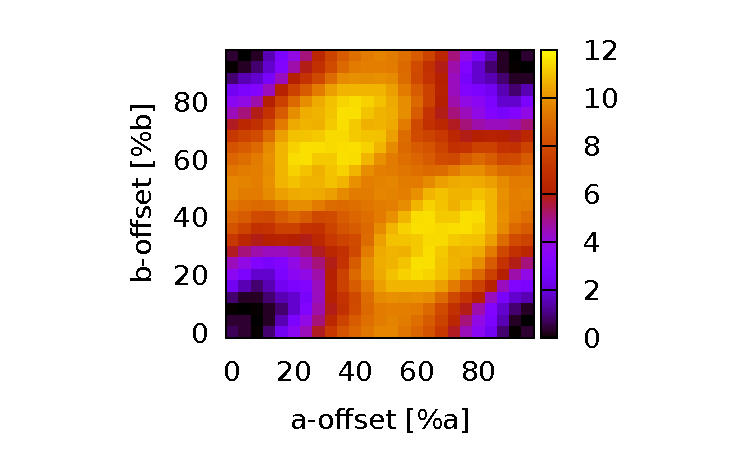
\includegraphics[trim={2cm 0cm 1.9cm 0.4cm},clip,width=8.5cm]{images/LJ_all_05000N2_map.pdf}& 
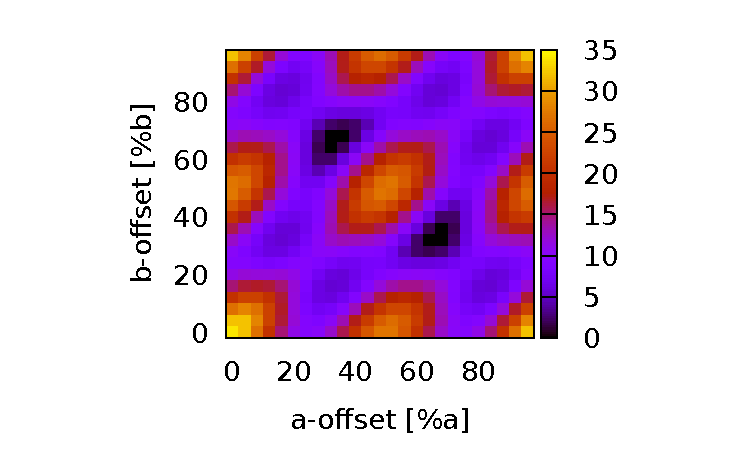
\includegraphics[trim={2cm 0cm 1.9cm 0.4cm},clip,width=8.5cm]{images/LAMMPS_all_05000N2_map.pdf}\\
\textbf{\Large{LJ}}\par\medskip & \textbf{\Large{LJ+Coul.}}\par\medskip\\
\multicolumn{2}{c}{ 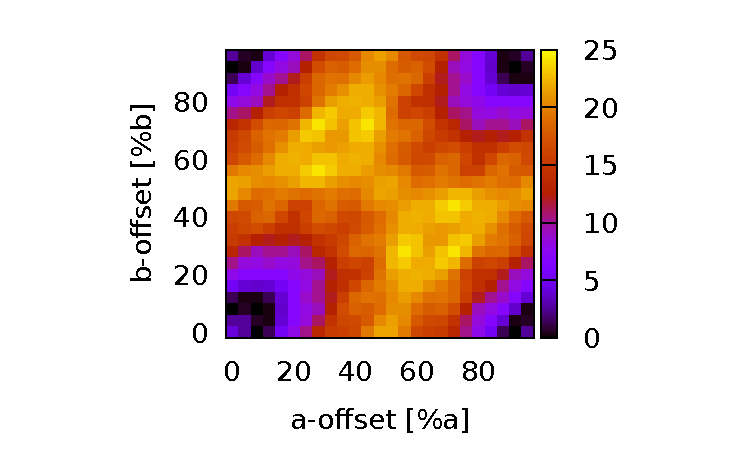
\includegraphics[trim={2cm 0cm 1.9cm 0.4cm},clip,width=8.5cm]{images/DFTB_all_05000N2_map.pdf}} \\ 
\multicolumn{2}{c}{\textbf{\Large{DFTB+}}\par\medskip}\\
\end{tabular}}
\caption{Mapping of the offset-dependent potential for COF 05000N2; for every x-y point, only the z-value leading to the lowest energy was kept; energy in $kcal/mol$}
\label{fig:50maps}
\end{figure}






\begin{figure}[H]
\vspace{2cm}
\begin{centering}
\textbf{\LARGE{05001N2}}\par\medskip
\end{centering}
\makebox[\textwidth][c]{
\begin{tabular}{cc}
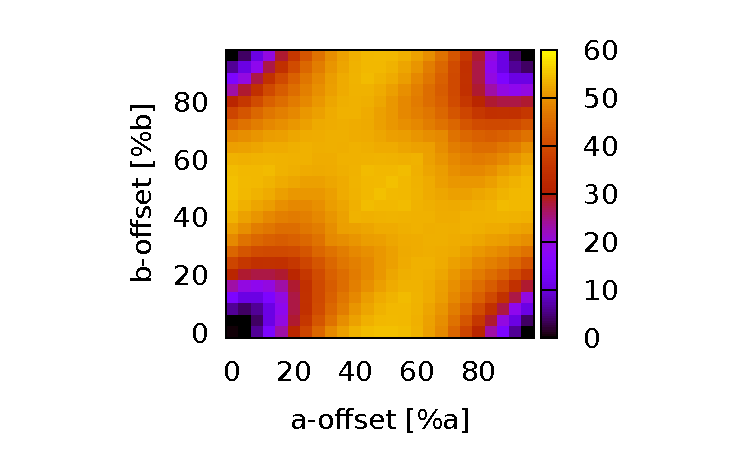
\includegraphics[trim={2cm 0cm 1.9cm 0.4cm},clip,width=8.5cm]{images/LJ_all_05001N2_map.pdf}& 
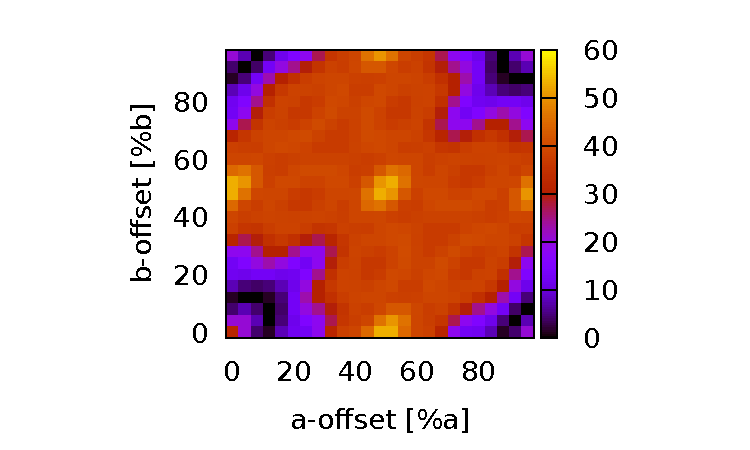
\includegraphics[trim={2cm 0cm 1.9cm 0.4cm},clip,width=8.5cm]{images/LAMMPS_all_05001N2_map.pdf}\\
\textbf{\Large{LJ}}\par\medskip & \textbf{\Large{LJ+Coul.}}\par\medskip\\
\multicolumn{2}{c}{ 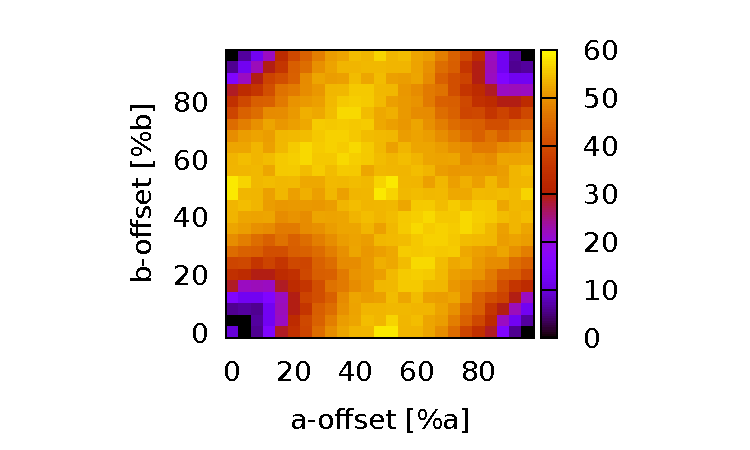
\includegraphics[trim={2cm 0cm 1.9cm 0.4cm},clip,width=8.5cm]{images/DFTB_all_05001N2_map.pdf}} \\ 
\multicolumn{2}{c}{ \textbf{\Large{DFTB+}}\par\medskip}\\
\end{tabular}}
\caption{Mapping of the offset-dependent potential for COF 05001N2; for every x-y point, only the z-value leading to the lowest energy was kept; energy in $kcal/mol$}
\label{fig:51maps}
\end{figure}







\begin{figure}[H]
\vspace{2cm}
\begin{centering}
\textbf{\LARGE{10000N2}}\par\medskip
\end{centering}
\makebox[\textwidth][c]{
\begin{tabular}{cc}
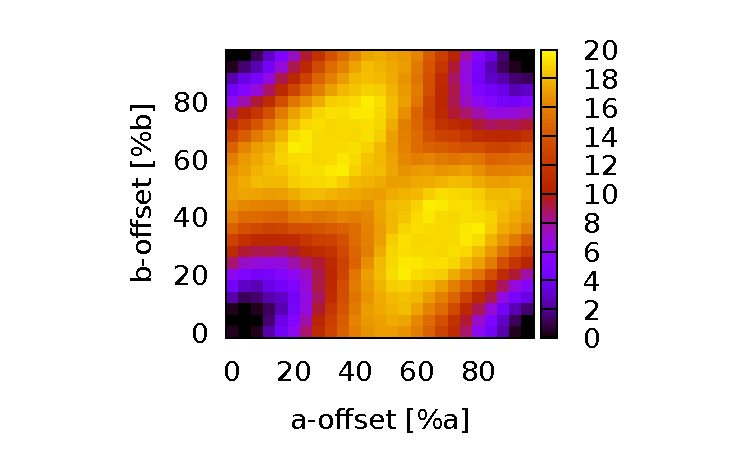
\includegraphics[trim={2cm 0cm 1.9cm 0.4cm},clip,width=8.5cm]{images/LJ_all_10000N2_map.pdf}& 
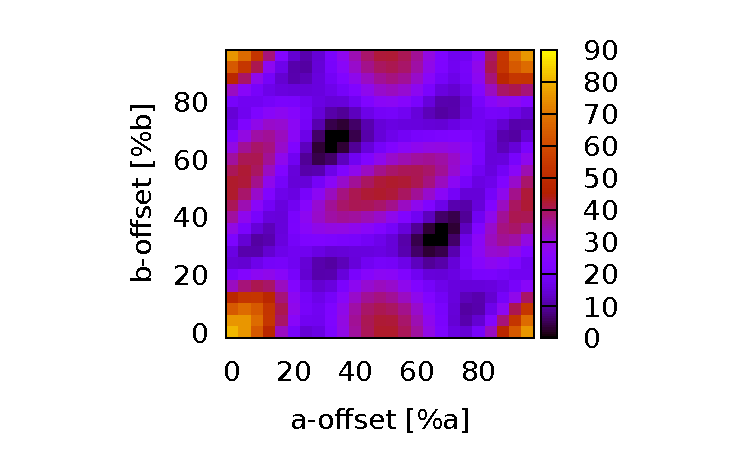
\includegraphics[trim={2cm 0cm 1.9cm 0.4cm},clip,width=8.5cm]{images/LAMMPS_all_10000N2_map.pdf}\\
\textbf{\Large{LJ}}\par\medskip & \textbf{\Large{LJ+Coul.}}\par\medskip\\
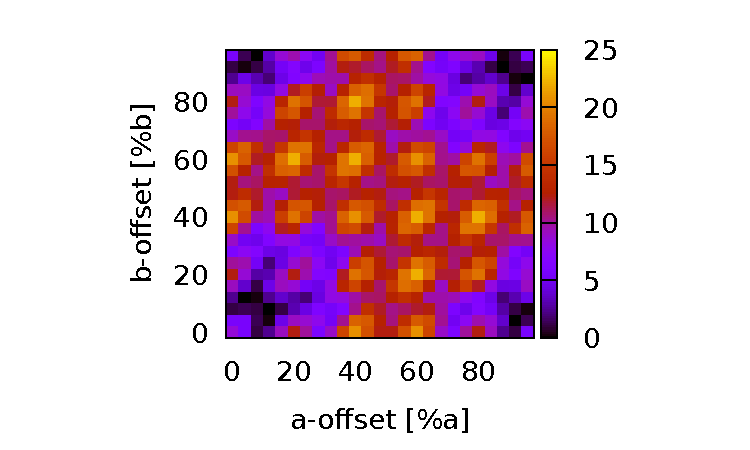
\includegraphics[trim={2cm 0cm 1.9cm 0.4cm},clip,width=8.5cm]{images/xTB_all_10000N2_map.pdf}& 
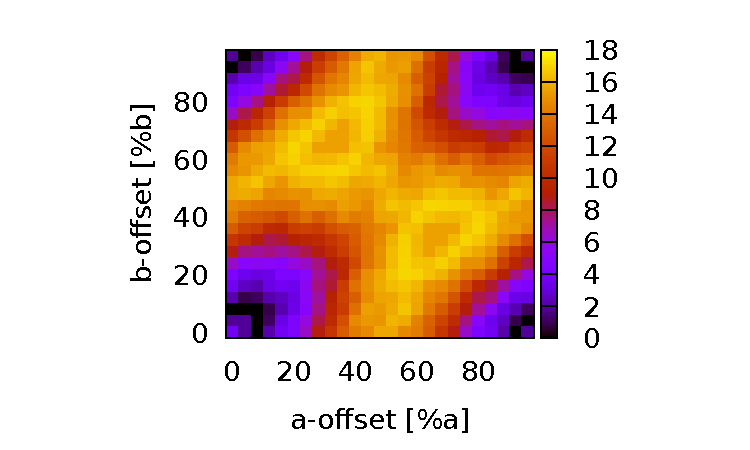
\includegraphics[trim={2cm 0cm 1.9cm 0.4cm},clip,width=8.5cm]{images/DFTB_all_10000N2_map.pdf} \\ 
\textbf{\Large{xTB}}\par\medskip & \textbf{\Large{DFTB+}}\par\medskip\\
\end{tabular}}
\caption{Mapping of the offset-dependent potential for COF 10000N2; for every x-y point, only the z-value leading to the lowest energy was kept; energy in $kcal/mol$}
\label{fig:10maps}
\end{figure}



\begin{figure}[H]
\vspace{2cm}
\begin{centering}
\textbf{\LARGE{13000N2}}\par\medskip
\end{centering}
\makebox[\textwidth][c]{
\begin{tabular}{cc}
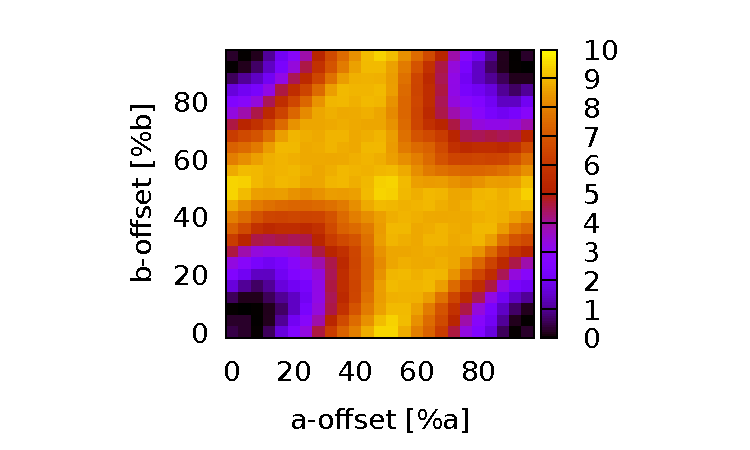
\includegraphics[trim={2cm 0cm 1.9cm 0.4cm},clip,width=8.5cm]{images/LJ_all_13000N2_map.pdf}& 
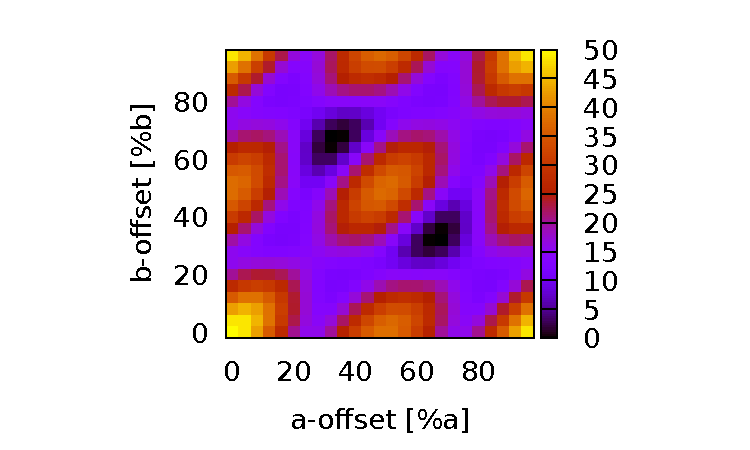
\includegraphics[trim={2cm 0cm 1.9cm 0.4cm},clip,width=8.5cm]{images/LAMMPS_all_13000N2_map.pdf}\\
\textbf{\Large{LJ}}\par\medskip & \textbf{\Large{LJ+Coul.}}\par\medskip\\
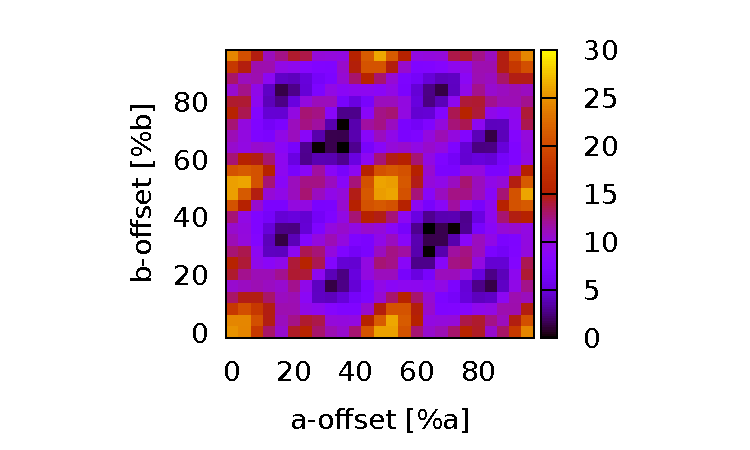
\includegraphics[trim={2cm 0cm 1.9cm 0.4cm},clip,width=8.5cm]{images/xTB_all_13000N2_map.pdf}& 
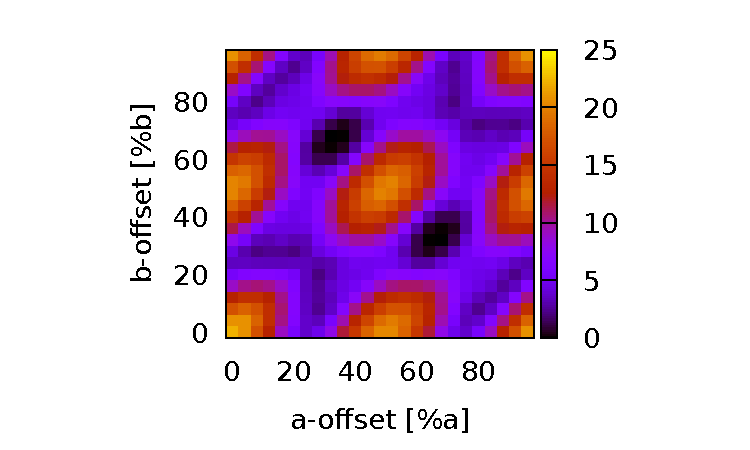
\includegraphics[trim={2cm 0cm 1.9cm 0.4cm},clip,width=8.5cm]{images/DFTB_all_13000N2_map.pdf} \\ 
\textbf{\Large{xTB}}\par\medskip & \textbf{\Large{DFTB+}}\par\medskip\\
\end{tabular}}
\caption{Mapping of the offset-dependent potential for COF 13000N2; for every x-y point, only the z-value leading to the lowest energy was kept; energy in $kcal/mol$}
\label{fig:13maps}
\end{figure}




\begin{figure}[H]
\vspace{2cm}
\begin{centering}
\textbf{\LARGE{17120N2}}\par\medskip
\end{centering}
\makebox[\textwidth][c]{
\begin{tabular}{cc}
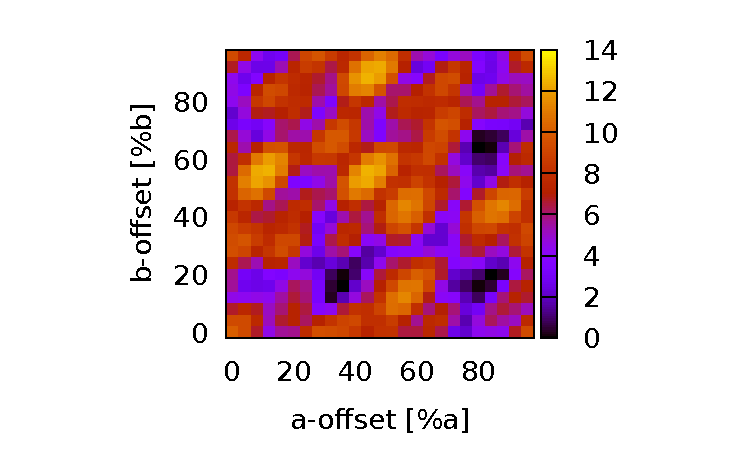
\includegraphics[trim={2cm 0cm 1.9cm 0.4cm},clip,width=8.5cm]{images/LJ_all_17120N2_map.pdf}& 
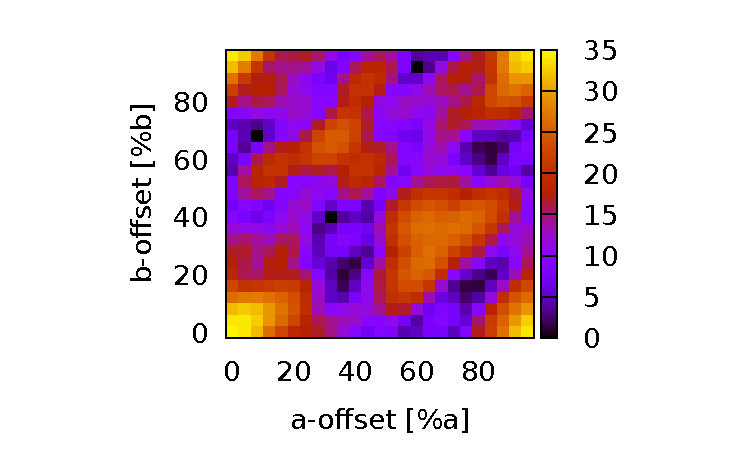
\includegraphics[trim={2cm 0cm 1.9cm 0.4cm},clip,width=8.5cm]{images/LAMMPS_all_17120N2_map.pdf}\\
\textbf{\Large{LJ}}\par\medskip & \textbf{\Large{LJ+Coul.}}\par\medskip\\
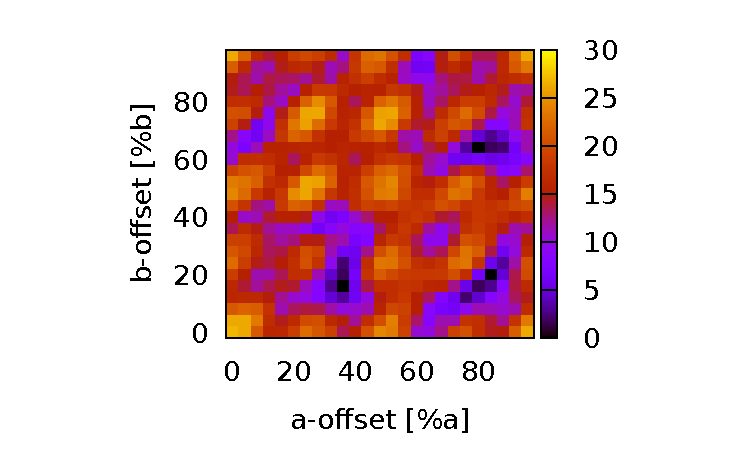
\includegraphics[trim={2cm 0cm 1.9cm 0.4cm},clip,width=8.5cm]{images/xTB_all_17120N2_map.pdf}& 
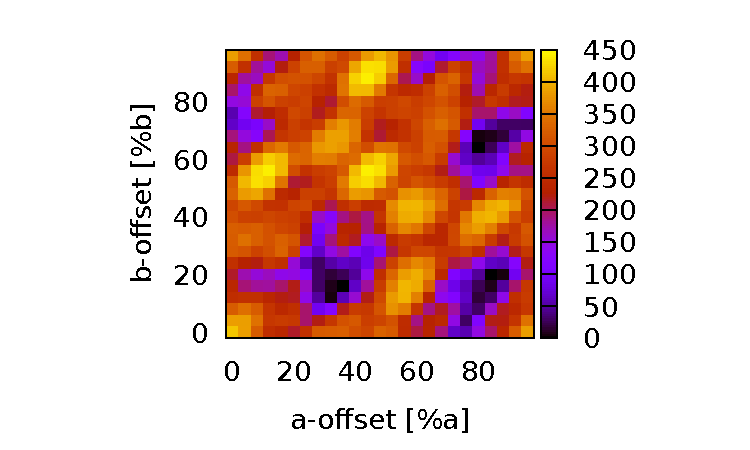
\includegraphics[trim={2cm 0cm 1.9cm 0.4cm},clip,width=8.5cm]{images/DFTB_all_17120N2_map.pdf} \\ 
\textbf{\Large{xTB}}\par\medskip & \textbf{\Large{DFTB+}}\par\medskip\\
\end{tabular}}
\caption{Mapping of the offset-dependent potential for COF 17120N2; for every x-y point, only the z-value leading to the lowest energy was kept; energy in $kcal/mol$}
\label{fig:17maps}
\end{figure}



\begin{figure}[H]
\vspace{2cm}
\begin{centering}
\textbf{\LARGE{18112N2}}\par\medskip
\end{centering}
\makebox[\textwidth][c]{
\begin{tabular}{cc}
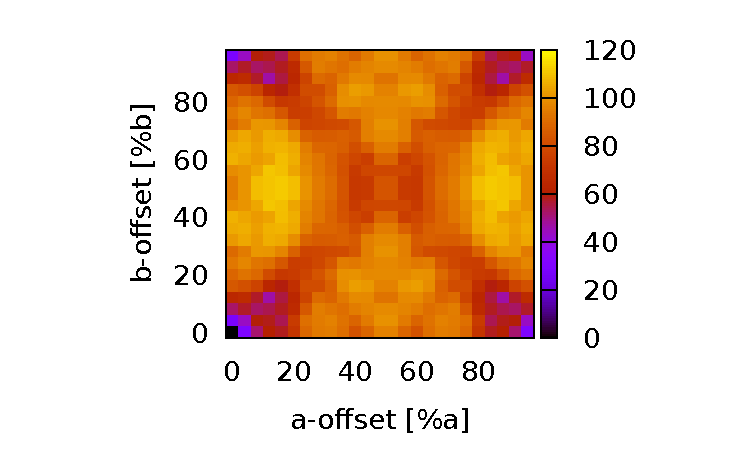
\includegraphics[trim={2cm 0cm 1.9cm 0.4cm},clip,width=8.5cm]{images/LJ_all_18112N2_map.pdf}& 
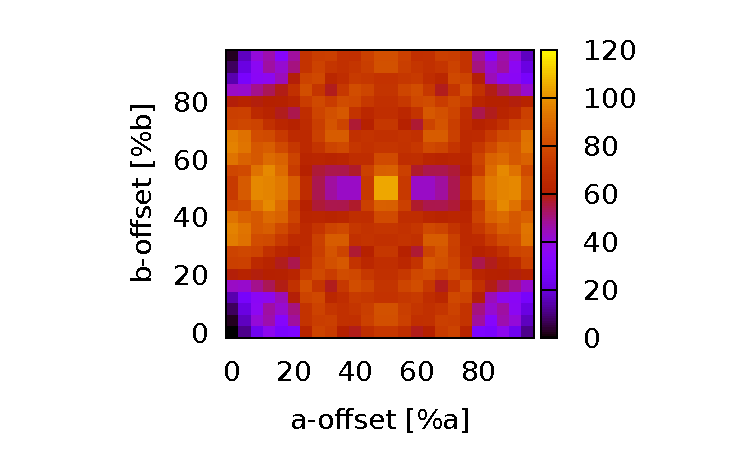
\includegraphics[trim={2cm 0cm 1.9cm 0.4cm},clip,width=8.5cm]{images/LAMMPS_all_18112N2_map.pdf}\\
\textbf{\Large{LJ}}\par\medskip & \textbf{\Large{LJ+Coul.}}\par\medskip\\
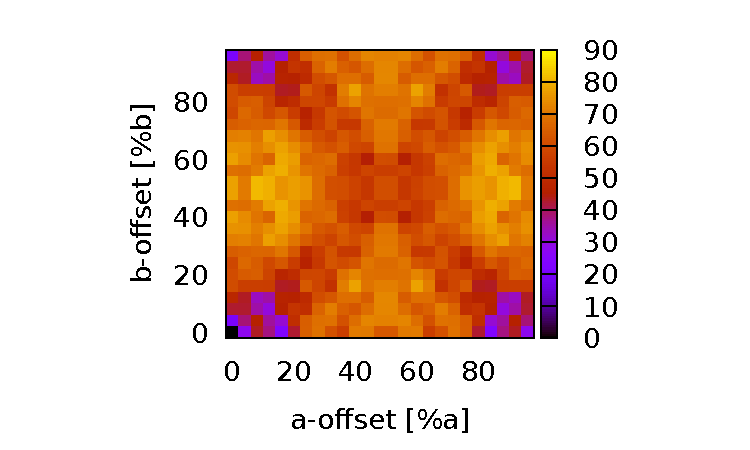
\includegraphics[trim={2cm 0cm 1.9cm 0.4cm},clip,width=8.5cm]{images/xTB_all_18112N2_map.pdf}& 
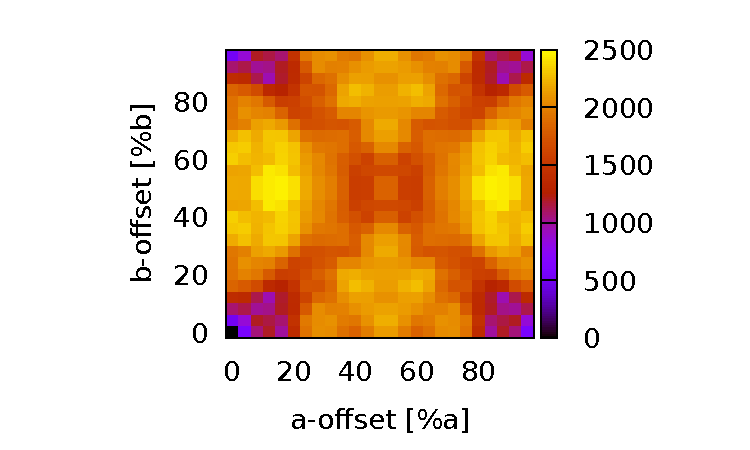
\includegraphics[trim={2cm 0cm 1.9cm 0.4cm},clip,width=8.5cm]{images/DFTB_all_18112N2_map.pdf} \\ 
\textbf{\Large{xTB}}\par\medskip & \textbf{\Large{DFTB+}}\par\medskip\\
\end{tabular}}
\caption{Mapping of the offset-dependent potential for COF 18112N2; for every x-y point, only the z-value leading to the lowest energy was kept; energy in $kcal/mol$}
\label{fig:18maps}
\end{figure}



\subsection{Limitations of CP2K xTB}
\label{sec:xTB_fail}
The implementation of xTB used in this project was the development version implemented on CP2K. Bugs were reported to us over the course of the project that explains the long runtime that was observed and could explain the regular grid-like pattern that appears on the PES. Because of the unstability of this program, the calculations using this method were abandoned over the course of the project. Nonetheless it would be interesting to re-iterate the experiment when a stable version of this program will be available.

\subsection{Influence of initial structure}

\subsection{Influence of point charge assignment method}

A crucial point in estimating the classical Coulombic interactions is the assignment of point-charges. Different methods were tested for that purpose. As a first estimation the EGULP charge equilibration routine was tested. The table below displays (see Figure \ref{fig:symetry}) the charge distribution over atoms and their mirror image along the a=b plane in the symmetric COF 13000N2. The charge distribution is compared to the Hirshfeld charges obtained using DFT. As one can see on the table below the charge repartition is strongly asymetric, which is an unphysical behavior (since a symmetric molecule must lead to an electron density having at least the same symmetries)
Furthermore some benzene-bounded Fluorine have positive point charges which, given the electron-donating abilities of benzene and the very strong electronegativity of Fluorine is unlikely. Hirshfeld point charge partition, although not perfectly symmetric, yield a much more reasonable charge repartition.
The asymetry could be caused by the very slight deviations to a perfect symmetry in the COF structure (>$10^{-3}\AA$). Indeed these are too slight to justify the  deviations observed with EGULP but could explain the ones observed with DFT.

%
\begin{figure}[H]
\begin{centering}
\textbf{Charge symmetry comparison}\par\medskip
\scalebox{0.7}{
\begin{tabular}{|c||c|c||c|c|}
\hline
Element & \multicolumn{2}{c||}{Egulp} &\multicolumn{2}{c|}{Hirshfeld}\\
\hline
\hline
C&0.325&0.414&0.275&0.275\\
\hline
C&0.201&0.08&0.009&0.009\\
\hline
C&0.324&0.423&0.276&0.275\\
\hline
C&0.205&0.088&0.009&0.009\\
\hline
C&0.417&0.375&0.309&0.309\\
\hline
F&-0.466&-0.432&-0.306&-0.304\\
\hline
C&0.49&0.505&0.311&0.31\\
\hline
F&-0.37&0.107&-0.312&-0.301\\
\hline
C&0.065&-0.296&0.308&0.307\\
\hline
F&-0.511&-0.48&-0.314&-0.305\\
\hline
C&0.418&0.376&0.31&0.309\\
\hline
F&-0.465&-0.437&-0.306&-0.306\\
\hline
C&0.492&0.49&0.311&0.307\\
\hline
F&-0.37&0.114&-0.309&-0.312\\
\hline
C&0.062&-0.304&0.31&0.307\\
\hline
F&-0.517&-0.479&-0.302&-0.305\\
\hline
N&-0.328&-0.179&-0.287&-0.279\\
\hline
N&-0.327&-0.186&-0.287&-0.287\\
\hline
\end{tabular}
}
\caption{Comparison of the symmetry of charge repartitions using different charge equilibration method for the symmetric COF 13000N2; every atom's charge is compared to its mirror image along the symmetry axis for each technique}
\label{fig:symetry}
\end{centering}
\end{figure}

\subsection{Influence of the stacking on the electronic structure}

The equilibrium electronic structure of a molecule is influenced by the electrical field surrounding it. Since COFs are polarized, they create an electrical field which, at short distance, could influence the electronic structure of the adjacent layers. In order to assess the need to equilibrate the charge density, for every stacking configuration, the Hirshfeld as computed by DFTB+ for every grid-point were compared for a subset of COFs. Key statistical values of this analysis are displayed on the table below (see Figure \ref{fig:chg_var}).

\begin{figure}[H]
\begin{centering}
\textbf{Charge variation analysis}\par\medskip
\scalebox{0.7}{
\begin{tabular}{|c||c|c|}
\hline
COF&$max(\Delta(Q(x,y,z)))$ &$\overline{\sigma(Q_i(x,y,z)}$\\
\hline
\hline
05000N2&0.372&0.03958\\
\hline
05001N2&0.275&0.01922\\
\hline
10000N2&0.438&0.04028\\
\hline
13000N2&0.403&0.11313\\
\hline
17120N2&0.612&0.04851\\
\hline
\end{tabular}
}
\caption{analysis of the changes in charge partition as a function of the offset where $max(\Delta(Q(x,y,z)))$ is the maximum observed difference of charge for a given element and $\overline{\sigma(Q(x,y,z)}$ is the average over all elements of the standard deviation computed for each element in the COF}
\label{fig:chg_var}
\end{centering}
\end{figure}



%\chapter{Tables and Figures}
In this chapter we will see some examples of tables and figures.

\section{Tables}
Let's see how to make a well designed table.

\begin{table}[tb]
\caption[A floating table]{A floating table.}
\label{tab:esempio}
\centering
\begin{tabular}{ccc}
\toprule
name & weight & food \\ 
\midrule
mouse	& 10 g	& cheese \\
cat	& 1 kg	& mice \\
dog	& 10 kg	& cats \\
t-rex	& 10 Mg	& dogs \\
\bottomrule 
\end{tabular}
\end{table}

The table~\ref{tab:esempio} is a floating table and was obtained with the following code:
\begin{lstlisting}
\begin{table}[tb]
\caption[A floating table]{A floating table.}
\label{tab:example}
\centering
\begin{tabular}{ccc}
\toprule
	name 	& weight & food	  \\ 
\midrule
	mouse	& 10  g	 & cheese \\
	cat		&  1 kg	 & mice	  \\
	dog		& 10 kg	 & cats   \\
	t-rex	& 10 Mg	 & dogs	  \\
\bottomrule 
\end{tabular}
\end{table}
\end{lstlisting}

\lipsum[1-2]


\section{Figures}
Let's see now how to put one or several images in your text.


\begin{figure}[tb] 
\centering 
\includegraphics[width=0.5\columnwidth]{galleria_stampe} 
\caption[A floating figure]{A floating figure (the lithograph \emph{Galleria di stampe}, of M.~Escher, got from \url{http://www.mcescher.com/}).}
\label{fig:galleria} 
\end{figure}

\begin{figure}[tb] 
\centering 
\includegraphics{some_vector_graphics.pdf} 
\caption[A floating figure]{A floating figure with text typeset in "Utopia Latex", a font provided in the template-folder for typesetting figures with greek characters. The text has been "outlined" for best compatibility with the repro during the printing.}
\label{fig:vector_graphics} 
\end{figure}


The figure~\ref{fig:galleria} is a floating figure and was obtained with the following code:
\begin{lstlisting}
\begin{figure}[tb] 
\centering 
\includegraphics[width=0.5\columnwidth]{galleria_stampe} 
\caption[A floating figure]{A floating figure ... }
\label{fig:galleria} 
\end{figure}
\end{lstlisting}


\lipsum[1-2]

\begin{figure}[tb]
\centering

\subfloat[Asia personas duo.]
{\includegraphics[width=.45\columnwidth]{lorem}} \quad
\subfloat[Pan ma signo.]
{\label{fig:ipsum}%
\includegraphics[width=.45\columnwidth]{ipsum}} \\
\subfloat[Methodicamente o uno.]
{\includegraphics[width=.45\columnwidth]{dolor}} \quad
\subfloat[Titulo debitas.]
{\includegraphics[width=.45\columnwidth]{sit}}
\caption[Tu duo titulo debitas latente]{Tu duo titulo debitas
latente.}
\label{fig:esempio}
\end{figure}

The figure~\ref{fig:esempio} is a floating figure and was obtained with the following code:
\begin{lstlisting}
\begin{figure}[tb]
\centering
\subfloat[Asia personas duo.]
{\includegraphics[width=.45\columnwidth]{lorem}} \quad
\subfloat[Pan ma signo.]
{\label{fig:ipsum}%
\includegraphics[width=.45\columnwidth]{ipsum}} \\
\subfloat[Methodicamente o uno.]
{\includegraphics[width=.45\columnwidth]{dolor}} \quad
\subfloat[Titulo debitas.]
{\includegraphics[width=.45\columnwidth]{sit}}
\caption[Tu duo titulo debitas latente]{Tu duo titulo debitas latente.}
\label{fig:esempio}
\end{figure}
\end{lstlisting}


\lipsum[3-8]

%\chapter{Mathematics}
In this chapter we will see some examples of mathematics.

\lipsum[1]

\section{Very important formulas}
\lipsum[2]

\begin{equation}\label{eqn:rate_eqns}
\frac{\textrm{d}}{\textrm{d}t}\left[
\begin{array}{l}
P_{\textit{0}} \\
P_{\textit{1}} \\
P_{\textit{T}}
\end{array}
\right] =
\left[
\begin{array}{l}
\frac{P_{\textit{1}}}{\tau_{\textit{10}}} + \frac{P_{\textit{T}}}{\tau_{\textit{T}}} - \frac{P_{\textit{0}}}{\tau_{\textit{ex}}} \\
- \frac{P_{\textit{1}}}{\tau_{\textit{10}}} - \frac{P_{\textit{1}}}{\tau_{isc}} + \frac{P_{\textit{0}}}{\tau_{\textit{ex}}} \\
\frac{P_{\textit{1}}}{\tau_{isc}} -  \frac{P_{\textit{T}}}{\tau_{\textit{T}}}
\end{array}
\right]
\end{equation}

\lipsum[3]


\begin{equation}\label{eqn:avgfluorescence}
\bar{I_{f}}(\vec{r})	 
	= \gamma(\vec{r}) \left(1 - \frac{\tau_{\textit{T}} P_{\textit{T}}^{{eq}}\left(1-\exp \left(-\frac{(T_p - t_p)}{\tau_{\textit{T}}}\right)\right)}{1-\exp\left(-\frac{(T_p - t_p)}{\tau_{\textit{T}}} + k_{\textit{2}} t_p\right)} \times \frac{\left(\exp\left(k_{\textit{2}} t_p\right)-1\right)}{t_p} \right) 
\end{equation}

\lipsum[3]

%\chapter{Another chapter}
Here you can see a citation: \cite{atc13}.

\lipsum[7]



%%%%%%%%%%%%%%%%%%%%%%%%%%%%%%%%%%%%%%%%%%%%%%
%%%%% TAIL: Bibliography, Appendix, CV
%%%%%%%%%%%%%%%%%%%%%%%%%%%%%%%%%%%%%%%%%%%%%%
%\appendix
\chapter{An appendix}

\lipsum[1]

\backmatter
%\cleardoublepage
\phantomsection
\bibliographystyle{plainnat}
\bibliography{tail/biblio.bib}
\addcontentsline{toc}{chapter}{Bibliography}


\printbibliography
% Add your glossary here
% Add your index here
% Photographic credits (list of pictures&images that have been used with names of the person holding the copyright for them)
%\cleardoublepage
\thispagestyle{empty}
\phantomsection
\addcontentsline{toc}{chapter}{Curriculum Vitae}
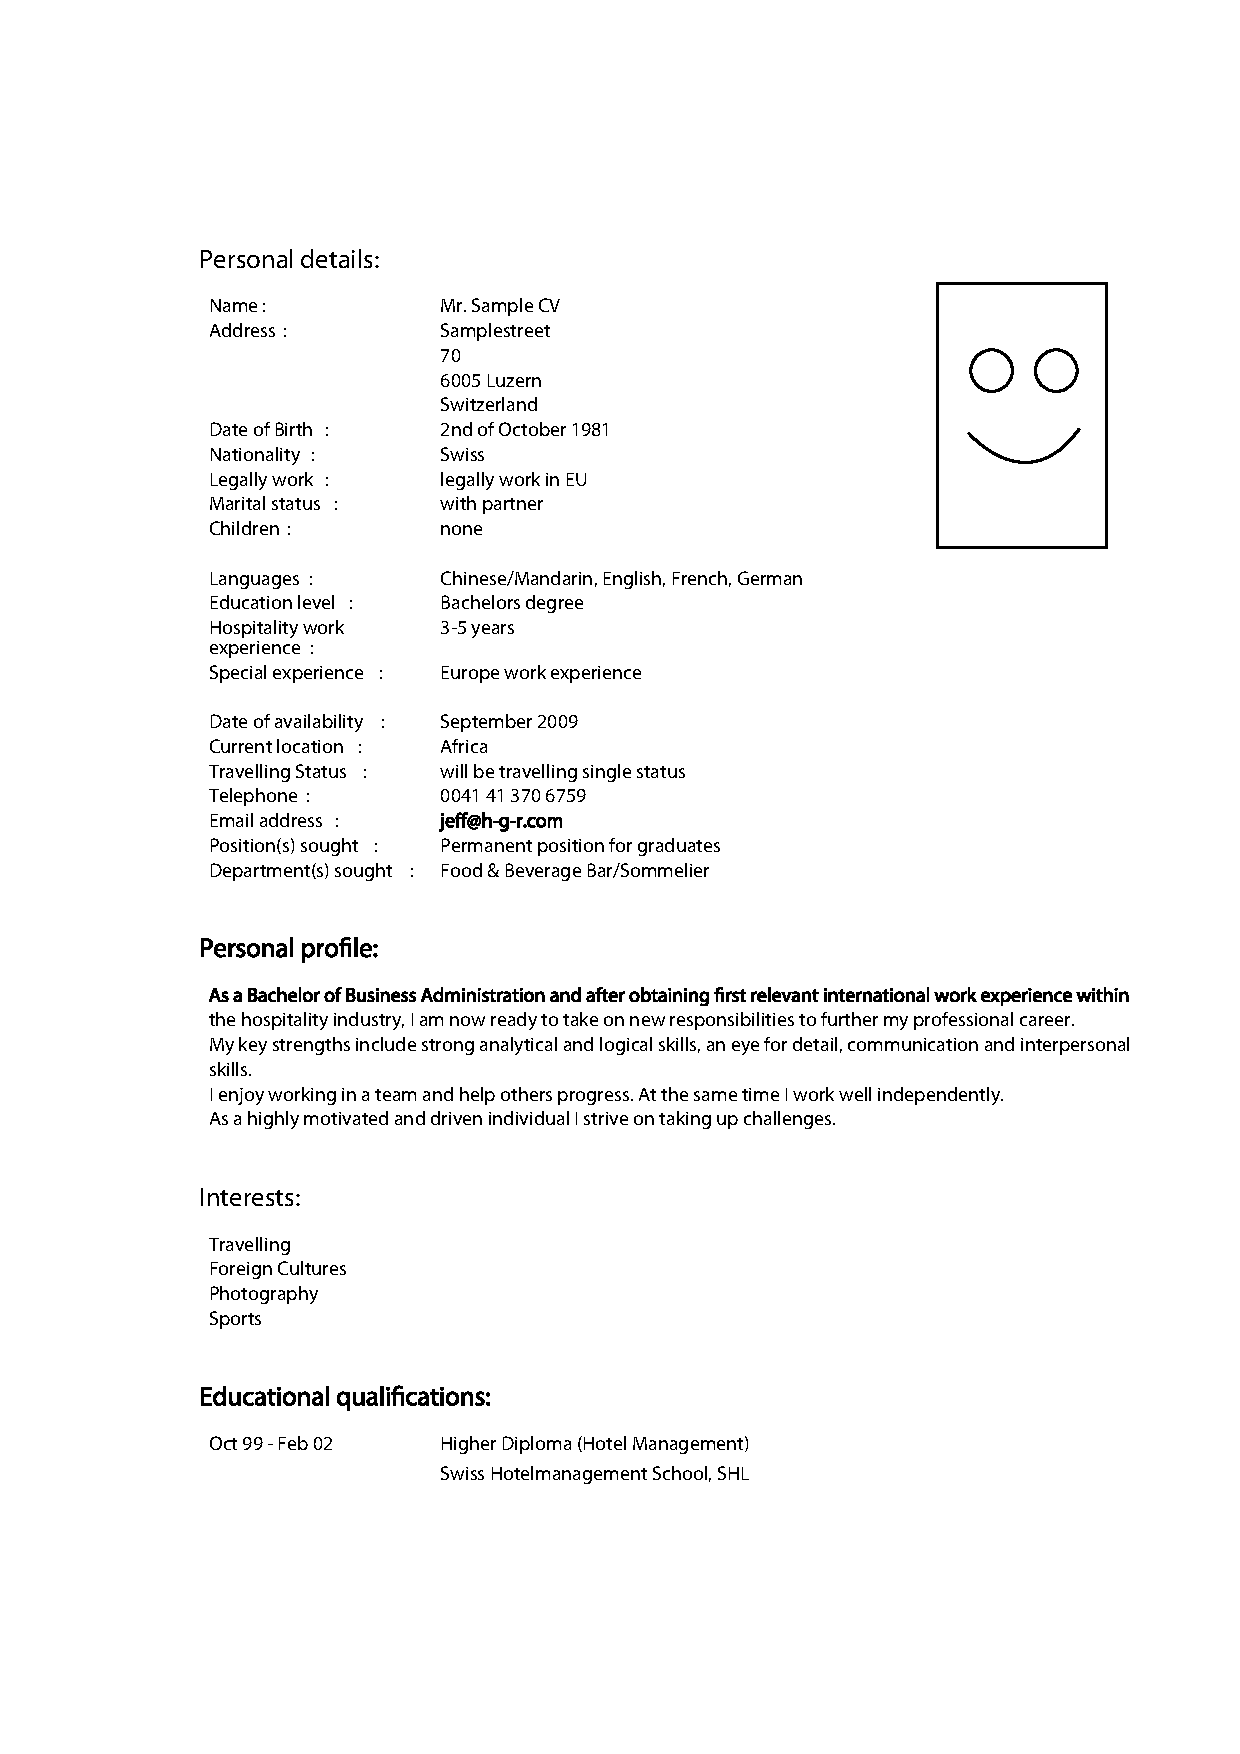
\includepdf[pagecommand=\thispagestyle{addpagenumbersforpdfimports},pages=-]{tail/cv.pdf}

\end{document}
